% last updated in April 2002 by Antje Endemann
% Based on CVPR 07 and LNCS, with modifications by DAF, AZ and elle, 2008 and AA, 2010, and CC, 2011; TT, 2014; AAS, 2016

\documentclass[runningheads]{llncs}
\usepackage[namelimits]{amsmath} 
\usepackage{amssymb}             
\usepackage{amsfonts}           
\usepackage{mathrsfs}            
\usepackage{graphicx}
\usepackage{amsmath,amssymb} % define this before the line numbering.
\usepackage{ruler}
\usepackage{color}
\usepackage[ruled]{algorithm2e}
\usepackage{multirow}
\usepackage{bm}

\newcommand{\BY}{{Y}}
\newcommand{\BA}{{\mathbf{A}}}
\newcommand{\BX}{{\mathbf{X}}}
\newcommand{\BXs}{{\mathbf{Xs}}}
\newcommand{\BLs}{{\mathbf{Ls}}}
\newcommand{\BD}{{\mathbf{D}}}
\newcommand{\BP}{{\mathbf{P}}}
\newcommand{\BL}{{\mathbf{L}}}
\newcommand{\Bone}{{\mathbf{1}}}
\newcommand{\BU}{{\mathbf{X}}}
\newcommand{\BS}{{\mathcal{S}}}
\newcommand{\BB}{{\mathbf{B}}}
\newcommand{\Bb}{{\mathbf{b}}}
\newcommand{\BR}{{\mathbf{R}}}
\newcommand{\BW}{{\mathbf{W}}}
\newcommand{\BE}{{\mathbf{E}}}
\newcommand{\Be}{{\mathbf{e}}}
\newcommand{\BZ}{{\mathbf{Z}}}
\newcommand{\BM}{{\mathbf{M}}}
\newcommand{\BQ}{{\mathbf{Q}}}
\newcommand{\BT}{{\mathbf{T}}}
\newcommand{\BI}{{\mathbf{I}}}
\newcommand{\T}{{\!\top}}
\newcommand{\Bx}{{\mathbf{x}}}
\newcommand{\By}{{\mathbf{y}}}

\newcommand{\etal}{{et al}}
\newcommand{\etc}{\textit{{etc}}}
\newcommand{\eg}{{e.g.}}
\newcommand{\ie}{{i.e.}}
\newcommand{\w}{{\mathrm{w}}}

\renewcommand{\Lambda}{\varLambda}
\newcommand{\st}{{\,\,\mathrm{s.t.\,\,}}}
\newcommand{\diag}{{\mathrm{diag}}}
\newcommand{\const}{{\mathrm{const.}}}
\newcommand{\trace}{{\mathrm{Tr}}}
\newcommand{\sgn}{{\mathrm{sgn}}}

\usepackage[width=122mm,left=12mm,paperwidth=146mm,height=193mm,top=12mm,paperheight=217mm]{geometry}
\begin{document}
% \renewcommand\thelinenumber{\color[rgb]{0.2,0.5,0.8}\normalfont\sffamily\scriptsize\arabic{linenumber}\color[rgb]{0,0,0}}
% \renewcommand\makeLineNumber {\hss\thelinenumber\ \hspace{6mm} \rlap{\hskip\textwidth\ \hspace{6.5mm}\thelinenumber}}
% \linenumbers
\pagestyle{headings}
\mainmatter
\def\ECCV18SubNumber{1917}  % Insert your submission number here

\title{Generative Domain-Migration Hashing for Sketch-to-Image Retrieval} % Replace with your title

\titlerunning{ECCV-18 submission ID \ECCV18SubNumber}

\authorrunning{ECCV-18 submission ID \ECCV18SubNumber}

\author{Anonymous ECCV submission}
\institute{Paper ID \ECCV18SubNumber}


\maketitle

\begin{abstract}
Due to the succinct nature of free-hand sketch drawings, sketch-based image retrieval (SBIR) has abundant practical use cases in consumer electronics. However, SBIR remains a long-standing unsolved problem mainly because of the significant discrepancy between the sketch domain and the image domain. In this work, we propose a Generative Domain-migration Hashing (GDH) approach, which for the first time generates hashing codes from synthetic natural images that are migrated from sketches. The generative model learns a mapping that the distributions of sketches can be indistinguishable from the distribution of natural images using an adversarial loss, and simultaneously learns an inverse mapping based on the cycle consistency loss in order to enhance the indistinguishability. With the robust mapping learned from the generative model, GDH can migrate sketches to their indistinguishable image counterparts while preserving the domain-invariant information of sketches. With an end-to-end multi-task learning framework, the generative model and binarized hashing codes can be jointly optimized. Comprehensive experiments of both category-level and fine-grained SBIR on multiple large-scale datasets demonstrate the consistently balanced superiority of GDH in terms of efficiency, memory costs and effectiveness. 



%Sketch-based image retrieval (SBIR) can be regarded as a challenging cross-domain retrieval problem since it is difficult to bridge the domain gap between images and free-hand sketches.
%To address such a problem, previous studies mainly focus on embedding the low-level images and sketches with high dimensions into a high-level common feature subspace with low dimensions. However, the projection from image domain and sketch domain into common subspace will lead to the information loss in both domains and undesirable retrieval results. 
%Moreover, the continuous value embedding features are time-consuming for distance computation. Inspired by CycleGANs, 
%In this paper, we propose a novel hashing model called Generative Domain-shift Hashing (GDH) for accurate and efficient SBIR. 
%Our GDH architecture contains two parts: the domain-shift networks and the hash network.
% The domain-shift parts networks can convert sketches into images
% convert sketch domain into image domain to bridge the domain gap and preserve the information of images and sketches as much as possible. 
% The hash net is able to generate compact binary codes for retrieval efficiency. 
%GDH first builds the strong connection between images and sketches via the domain-shift networks.
%Different from previous works which inevitably causes the information loss in both image and sketch domains, our domain-shift networks embed sketches  into images since image domain carries more information.
%With the conversion from sketches into images, we solve the cross-domain hashing problem by a multi-task and end-to-end generative adversarial learning architecture. The proposed GDH approach is a universal framework which can effectively incorporate category-level and fine-grained retrieval tasks. 
%To our best knowledge, this work is the first hashing work which solves the SBIR problem by shifting the sketch domain into image domain. And it is the first work to incorporates category-level and fine-grained retrieval into a unified framework.
%Comprehensive experiments on the TU-Berlin Extension and Sketchy datasets demonstrate the superiority of GDH compared with both binary and real-valued state-of-the-art cross-modality methods in terms of retrieval precision and resource usage.
%achieves better performance compared to state-of-the-art 
%While our binary results of fine-grained retrieval experiments are competitive. 
 

\keywords{Domain-migration $\cdot$ Hash function $\cdot$ SBIR}
\end{abstract}
\section{Introduction}
% With the prevalence of modern touchscreen devices, sketch-based image retrieval (SBIR) \cite{SaavedraB10,sketchanet,2012sketchhash,Yu2016shoes,SangkloyBHH16,SongYSXH17,EitzHBA10} has attracted increasing attention. Suppose that you want to retrieve an image, however, unfortunately, you just forget the keywords of the image or the objects in the image is hard to be described. Under this circumstance, It is a good choice that using a sketch to 
% retrieve it. 
% %SBIR works can be categorized into two categories: category-level SBIR and fine-grained SBIR. 
% Many works have been done to address such a problem. Compared to traditional retrieval method content-based image retrieval (CBIR) and text-based image retrieval (TBIR),
% SBIR attaches more importance to location, shape, pose and other fine-grained details, which is much more convenient than describing it with hundreds words in text.
The prevalence of touchscreen in consumer electronics (range from portable devices to large home appliance) facilitates human-machine interactions free-hand drawings. The input of sketches is succinct, convenient and efficient for visually recording ideas, and can beat hundreds of words in some scenarios. As an extended application based on sketches,  sketch-based image retrieval (SBIR) \cite{SaavedraB10,sketchanet,2012sketchhash,Yu2016shoes,SangkloyBHH16,SongYSXH17,EitzHBA10} has attracted increasing attention. 

%fine-grained SBIR: preserve the geometrical morphology and detailed characteristic 


The primary challenge in SBIR is that free-hand sketches are inherently abstract and iconic, which magnifies cross-domain discrepancy between sketches and real-world images. Recent works attempt to employ cross-view learning methods \cite{SaavedraB10,EitzHBA10,LiuSSLS17,SaavedraB15,hu2010,ParuiM14,dalal2005,hu2010_1,Saavedra14,Lowe99} to address such a challenge, where the common practice is to reduce the domain discrepancy by embedding both sketches and natural images to a common space and use the projected features for retrieval. The most critical deficiency of this line of approaches is the learned mappings within each domain cannot be well-generalized to the test data, especially for categories with large variance. Similar to other image-based retrieval problems, the query time grows increasingly with the database size and exponentially with the dimension of sketch/image representations. To this end, Deep Sketch Hashing (DSH) \cite{LiuSSLS17} is introduced to replace the full-precision sketch/image representations with binary vectors. However, the quantization error introduced by the binarization procedure can destroy both domain-invariant information and the semantic consistency across domains. 


In this work, our primary goal is to improve deficiencies in aforementioned works and provide a practical solution to the scalable SBIR problem. We propose a Generative Domain-migration Hashing (GDH) method that improves the generalization capability by migrating sketches into the natural image domain, where the distribution migrated sketches can be indistinguishable from the distribution of natural images. Additionally, we introduce an end-to-end multi-task learning framework that jointly optimizes the cycle consistent migration as well as the hash codes, where the adversarial loss and the cycle consistency loss can simultaneously preserve 
the semantic consistency of the hashing codes. GDH also integrates an attention layer that guides the learning process to focus on the most representative regions.

While SBIR aims to retrieve natural images that shares identical category labels with the query sketch, fine-grained SBIR aims to preserve the intra-category instance-level consistency in addition to the category-level consistency. For the consistency purpose, we refer to standard SBIR as category-level SBIR and the fine-grained version as fine-grained SBIR respectively throughout the paper. Since the bidirectional mappings learned in GDH are highly under-constrained (\emph{i.e.}, does not require the pixel-level alignment \cite{IsolaZZE17} between sketches and natural images), GDH can naturally provide an elegant solution for preserving the geometrical morphology and detailed instance-level characteristic between sketches and natural images. In addition, a triplet ranking loss is introduced to enhance the fine-grained learning based on visual similarities of intra-class instances. The pipeline of the proposed GDH method for both category-level and fine-grained SBIR tasks is illustrated in Fig. \ref{fig:overview}. Extensive experiments on various large-scale datasets for both category-level and fine-grained SBIR tasks demonstrate the consistently balanced superiority of GDH in terms of memory cost, retrieval time and accuracy. The main contributions of this work are as follows:
%Nevertheless, SBIR is a very challenging problem. First, free-hand sketches are drawn with little reference. Compared to natural images, the shape and scale are often distorted, making 
%sketches distinctly more abstract than edge maps. Second, there is a huge domain gap between sketches and natural images since a sketch mainly contains the information of shape and structure and contains no information about color and texture. To solve these problems, many methods based on cross-domain retrieval are proposed. And we will discuss these methods for
%category-level SBIR and fine-grained SBIR respectively. Here, category-level SBIR means giving a sketch, retrieve images from same category as the sketch. Fine-grained SBIR means retrieve an image which corresponds to the query sketch. 

%For category-level SBIR, many methods \cite{LiuSSLS17,SaavedraB15,EitzHBA10,hu2010,ParuiM14,dalal2005,hu2010,hu2010_1,Saavedra14,SaavedraB10,Lowe99} focus on preserving the semantic information between the two domains by embedding both sketches and natural images to a common space. And these methods can be divided into two groups: hand-crafted methods and deep learning-based method.
%By detecting the edge or contour maps, hand-crafted methods first generate ``approximate sketches'' from natural images. 
%And then, SIFT \cite{Lowe99},
%HOG \cite{dalal2005}, gradient field HOG \cite{hu2010,hu2010_1}, histogram of edge local orientations (HELO) \cite{Saavedra14,SaavedraB10} and Learned Key Shapes(LKS) \cite{SaavedraB15} are applied to extracted the hand-crated features from sketches and ``approximate sketches''. 
%And then, the hand-crafted features are used to generate the SBIR representations. 
%Deep learning-based methods\cite{Yu2016shoes,LiuSSLS17,SongYSXH17,BuiRPC16} are further proposed, which apply multi-branch networks to feature embedding
%and achieve better performance than hand-crafted methods. Specifically, \cite{LiuSSLS17} proposes multi-branch networks named DSH to embed both sketches and images into binary space and
%achieve state-of-the-arts.
%However, the main limitation of DSH is that the domain gap between sketches and natural images is not well bridged. 
%Since embedding sketches and images to a common subspace may cause information loss in both domains and there is no constraint in DSH to control such loss which will
 %lead to undesirable retrieval results. In addition, DSH can not be effectively applied to fine-grained SBIR since it is specifically designed for category-level SBIR, and its common feature embedding space can not preserve the fine-grained detail information.
%And can not be well applied to fine-grained retrieval task.
%To cope with this problem, we propose our GDH which contains two mapping functions: $Image \rightarrow Sketch $ and $Sketch \rightarrow Image $. Apart from  two standard Adversarial
%loss respectively for $Image$ and $Sketch$, there are two corresponding consistency losses which are formulated by $L_1$ norm. Since the consistency loss constrains the fake image to real sketch, and the image domain carries more information than sketch domain, we can embed the sketch domain into image domain with little information loss.
%By doing so, we turn the cross-domain problem into a single domain problem.
%Hence, different from DSH and the other methods, our model only have one hash net and achieve better performance. 

%For fine-grained SBIR methods \cite{SangkloyBHH16,Yu2016shoes,BuiRPC16,SongYSXH17}, the overall triplet architectures which consist of multi-branch deep convolutional neural networks are quite similar. \cite{Yu2016shoes} proposes multi-branch networks with triplet ranking loss.
%In this case, the triplet inputs
%contain a sketch, a hard positive image corresponding to the sketch and a negative dissimilar image to the sketch. 
%The triplet loss is designed to pull matching pairs of photos and sketches close and push mis-matched pairs away. 
%And each branch embeds the corresponding inputs to a common feature subspace which preserves the semantic information and fine-grained details.
%However, the limitation is the same: the domain gap is not well bridged. And, searching efficiency of SBIR is lack of study. The multi-branch networks of \cite{Yu2016shoes} 
%produce continuous value features which are less
%memory efficiency and time-consuming.
%Furthermore, 
%since the domain-migration networks we proposed can effectively narrow the domain gap for both category-level and fine-grained retrieval,our GDH architectures are able to unify category-level retrieval and fine-grained retrieval into a single framework, and achieve higher 
%performance, lower memory complexity and less time-cost.
%However, there are still many challenges for deep learing-based SBIR methods. 
%First, find a commom feature space for sketches and images may not always perform well. The multi-branch
%deep architectures are difficult to keep all the domain-invariant features and the information loss will happend both 
%image domain and sketch domain, which results in the undesirable performance. 
%Second, most methods require simple datasets whose image contains only one object on a clean background for high performance. This is unpractical, for the natural images may 
%appear from different viewpoints with complex background. 
%Third, No method unifies category-level retrieval and fine-grained retrieval into a single framework.

%The main contributions of our
%works are three-fold:
%And these nearst neighbor(NN) searches based methods are also high computational complexity.  
%In this paper, we propose a novel \textit{Deep Generative Hashing for Sketch-based Image Retrieval} (GDH) framework for the fast SBIR task,
%which incorporates category-level retrieval and fine-grained retrieval into a unified framework. 
%Different to previous multi-branch architectures which embeds each inputs to the corresponding domain, 
%the CycleGANs part in our GDH model generates fake image from its corresponding sketch.
%Consequently, we embed the sketch domain into image domain with little information loss and the domain gap is bridged. And then,
%the hash function part in our GDH model learns the binary representation from the image and the fake image generated by its corresponding
%sketch. Our mainly contributions are three-fold:
%\vspace{-0.58em}
\begin{itemize}
  \item 
  \vspace{-0.589em}
    We for the first time propose a generative model GDH for the hashing-based SBIR problem. Comparing to existing methods, the generative model can essentially improve the generalization capability by migrating sketches into their indistinguishable counterparts in the natural image domain.
    %We put forward a novel joint end-to-end deep learning method GDH for both category-level
    %and fine-grained SBIR. GDH is able to solve the SBIR problem by 
    %migrating the sketch domain to image domain.
    %To our best knowledge, this work is the first hashing work which transfer
    %sketch domain to image domain with GANs for SBIR problems. And it is the first to incorporates
    %category-level retrieval 
    %and fine-grained retrieval into a unified framework.
  \item Guided by an adversarial loss and a cycle consistency loss, the optimized binary hashing codes can preserve the semantic consistency across domains. Meanwhile, training GDH does not require the pixel-level alignment across domains, and thus allows generalized and practical applications.
    %A novel multi-task deep architecture, which collaboratively addresses
%domain-migration and binary coding, is proposed based on discrete alternating iteration.
%Different from previous works contains multi-branch networks, our domain-migration networks are specifically designed. We use the generative network and the hash network for retrieval tasks, which is much simpler and faster.
%Particularly, sketches are fed into the network first to generate the corresponding fake images with little information loss, and the 
%hash function embeds the images and fake images into binary representations. As such, the GDH can better 
%narrow the domain gap between image domain and sketch domain compared to previous SBIR deep nets. And improve the 
%etrieval speed. 
  \item 
  GDH can improve the category-level SBIR performance over the state-of-the-art hashing-based SBIR method DSH \cite{LiuSSLS17} by up to $20.5\%$ on the TU-Berlin Extension dataset, and up to $26.4\%$ on the Sketchy dataset respectively. Meanwhile, GDH can achieve comparable performance with real-valued fine-grained SBIR methods, while significantly reduce the retrieval time and memory cost with binary codes. 
  
 \end{itemize}
% \begin{figure*}[t]
%     \centering
%     \includegraphics[width = 1\textwidth]{figures/sketch2image.pdf}
%     \caption{The visualization of our CycleGANs' outputs: sketches to images and images to sketches. (More examples can be seen in our supplementary documents)}
%     \label{fig:finegrained-figure}
% \end{figure*}

\begin{figure*}
\vspace{-5ex}
    \centering
    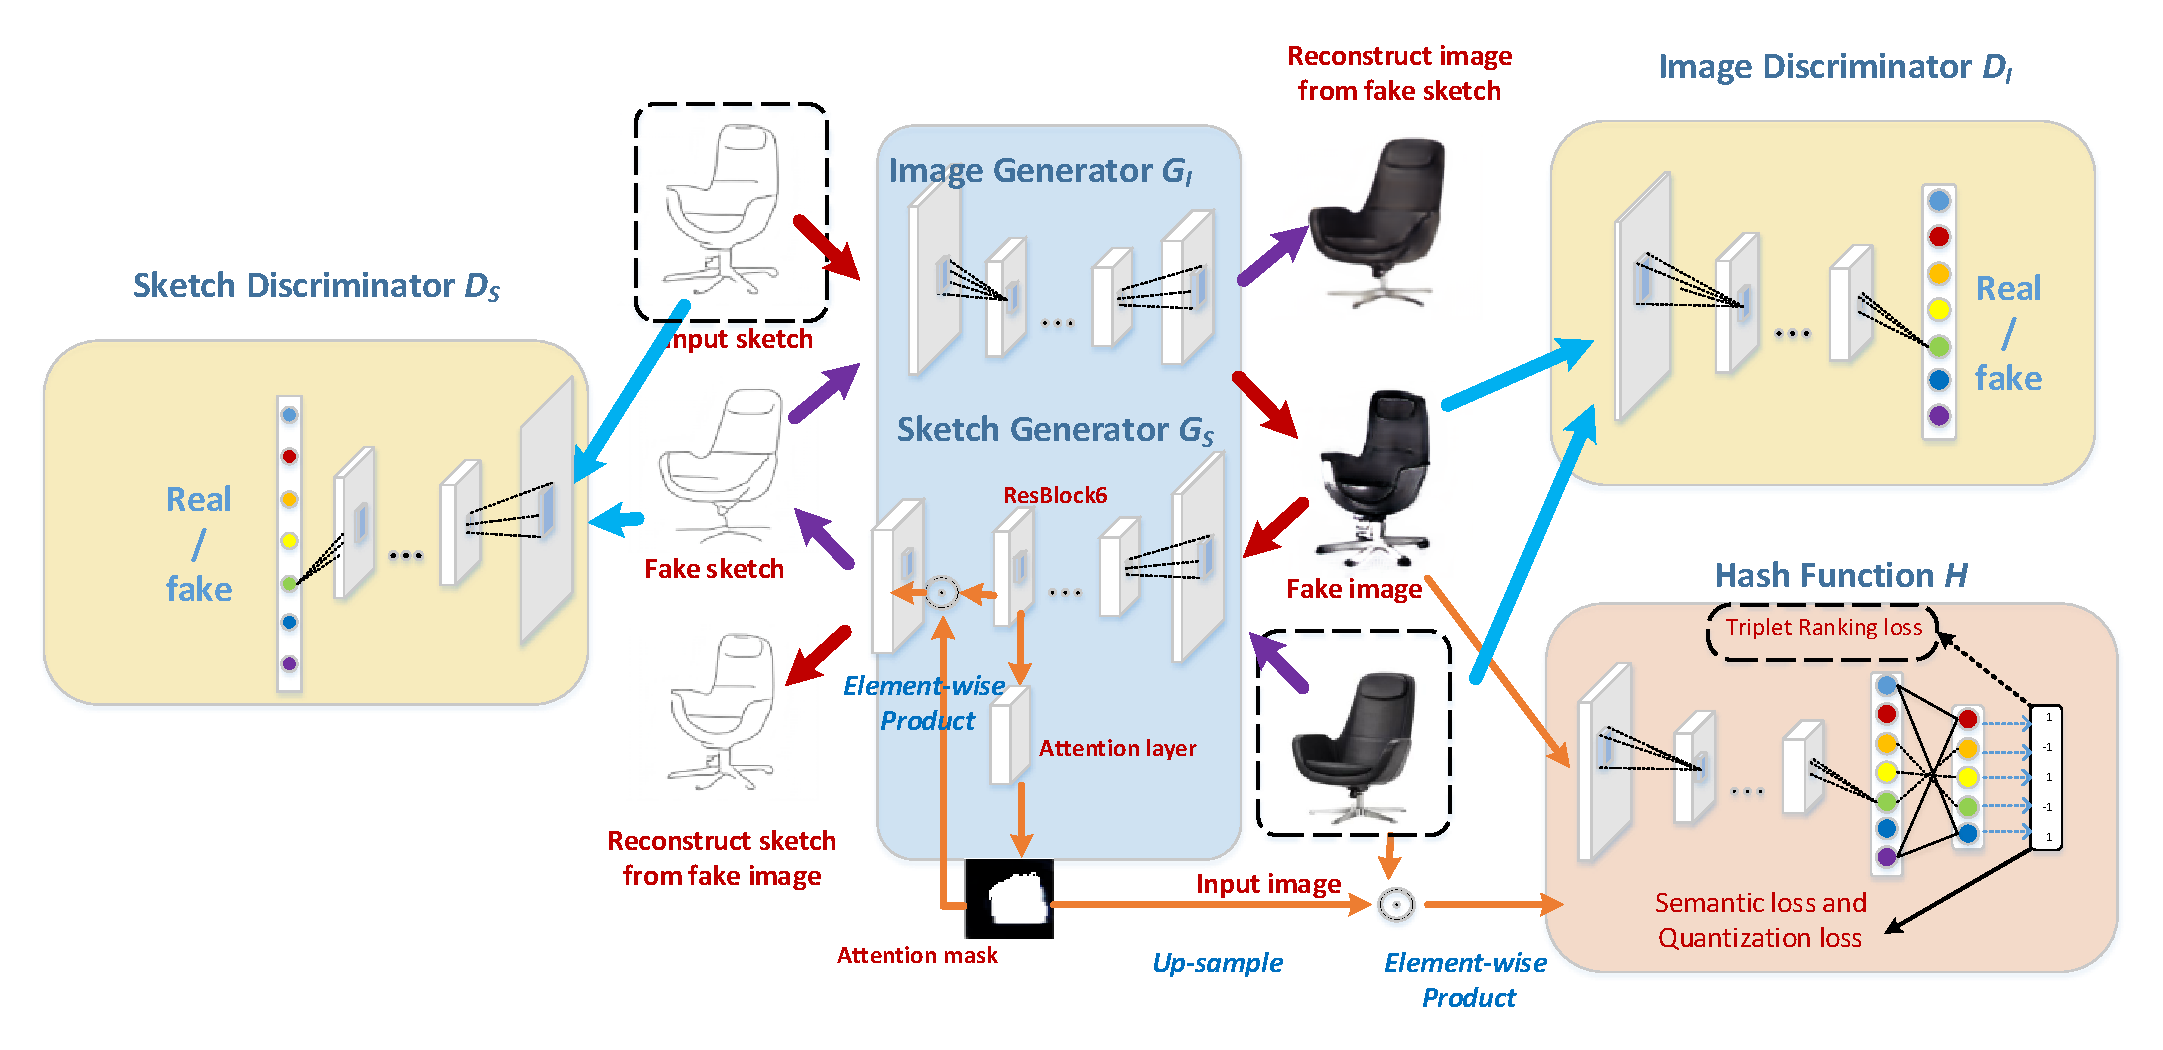
\includegraphics[width = 0.9\textwidth]{figures/overview2.pdf}
    \vspace{-3ex}
    \caption{Illustration of our deep model for the domain-migration networks and compact binary codes learning. The domain-migration module  consists of $G_I$, $G_S$, $D_I$ and $D_S$. The bottom right module is the hashing network $H$. The red arrows represent the cycle between real sketches and fake natural while the purple arrows represent the cycle between real natural images and fake sketches.}
    %Illustration of our deep model for the domain-shift networks and compact binary code learning. Sketches and images are fed into the domain-shift networks to train the generators $G_I$ and $G_S$ with a high quality. The top right part is the hash function $H$ with the input of real images and fake images with the calculation of the semantic loss (triplet ranking loss for fine-grained retrieval) and the quantization loss.
    \label{fig:overview}
    \vspace{-5ex}
\end{figure*}

\section{Related Work}
In this section, we discuss the following four directions of related works. 

\noindent\textbf{Category-level SBIR:} The majority of existing category-level SBIR methods \cite{SaavedraB10,EitzHBA10,LiuSSLS17,SaavedraB15,hu2010,ParuiM14,dalal2005,hu2010_1,Saavedra14,Lowe99,LiHSG14} rely on learning a common feature space for both sketches and natural images. However, learning such a common feature space based on the  can end up with an overfitting solution to the training data.

\noindent\textbf{Hashing-based SBIR:} If the learned common feature space is real-valued, the retrieval time depends on the database size, and the scalability of the algorithms can be consequently restrained. In order to to improve the efficiency, hashing-based methods \cite{DH15cvpr,liu2014discrete,KSH2012,shen2015supervised,SH08,zhang2016efficient,shen2017tmm,qin2017action,liu2017coding} are introduced to solve the SBIR problem. The state-of-the-art hashing-based SBIR method DSH \cite{liu2017coding} employed an end-to-end semi-heterogeneous CNNs to learn binarized hashing codes for retrieval. However, the generalization issue remains in DSH since the learned semi-heterogeneous CNNs are also non-linear mappings across the two domains.


\noindent\textbf{Generative Adversarial Networks:} The success of Generative Adversarial Networks (GANs) \cite{goodfellow2014generative} in various image generation \cite{denton2015deep} and representation learning \cite{mathieu2016disentangling} tasks is inspiring in a way that sketches can be migrated into the natural image domain using the adversarial loss, where the migrated sketches cannot be distinguished from natural images.  Image-to-image translation methods \cite{sangkloy2017scribbler,pix2pix2017} can serve this purpose and are capable of migrating sketches into natural images, however, the pixel-level alignment between each sketch and image pair required for training are impractical. In order to address such an issue,  Zhu et al. \cite{ZhuPIE17} introduced a cycle consistency loss. In this work, we employ such a cycle consistency loss and force the bidirectional mappings to be consistent with each other. Benefiting from the highly under-constrained cycled learning, sketches can be migrated to their indistinguishable counterparts in the natural image domain. 


\noindent\textbf{Fine-grained SBIR:} Among a limited number of fine-grained SBIR methods \cite{Yu2016shoes,SangkloyBHH16,SongYSXH17,BuiRPC16,XuYHSMWXKG18,LiPSHZH16,QiSZL16,XuYQSMWG16,LiPSHXZ17}, Yu et al. \cite{Yu2016shoes} proposed the multi-branch networks with triplet ranking loss, which preserved the visual similarities of intra-class sketch and natural image instances. In our work, we also exploit the triplet ranking loss for preserving the visual similarity of intra-class instances. With improved generalization capability to the test data and the binarized hashing codes, the proposed GDH method can achieve comparable performance with \cite{Yu2016shoes} on the fine-grained SBIR task, while requiring much less memory and retrieval time. 

%Most existing SBIR works \cite{LiuSSLS17,EitzHBA10,ParuiM14,2012sketchhash} focused on category-level sketch-to-image retrieval. In the meantime, the fine-grained SBIR problem was tackled by the deep learning architecture which can learn both feature representations and cross-domain matching functions jointly. Recently, some SBIR works \cite{TsengLCH12,FuruyaO14} are combined with hashing methods \cite{DH15cvpr,liu2014discrete,KSH2012,shen2015supervised,SH08,zhang2016efficient,shen2017tmm,qin2017action,liu2017coding} for efficient retrieval. Apart from using single-domain hashing, the SBIR problem can also be dealt with through cross-domain hashing techniques \cite{FuruyaO14,JiangL17,LinDH015,ZhangL14,KumarU11,BronsteinBMP10,DingGZ14,ViaSP05,XiePX14}. However, these methods which embed the sketches and images into a common semantic space will lead to the information loss in both domain and unpromising retrieval results.
%GANs \cite{GoodfellowPMXWOCB14,ZhuPIE17,LuTT17,BousmalisSDEK17} provided a suitable solution to such cross-migration problem. Zhu et al. \cite{ZhuPIE17} proposed a new type of GAN called CycleGAN to learn image-to-image
%translation from a source domain $X$ to a target domain $Y$ by taking the reconstruction error into account. Furthermore, Lu et al. \cite{LuTT17} proposed Conditional CycleGANs for face image generation.  Unfortunately, these methods are not specifically designed for SBIR and neglect the intrinsic relationship between freehand sketches and natural images, resulting in unsatisfactory performance and less searching efficiency.% Guo et al. \cite{GuoLWLWL17} proposed conditional GANs for SBIR. However, it is also real-valued multi-branch networks and its feature embedding strategy is not effective, leading to undesirable performance and less searching efficiency.

%In the next section, we will introduce our deep architectures and then elaborate on our objective function.

% \begin{figure*}[t]
%     \centering
%     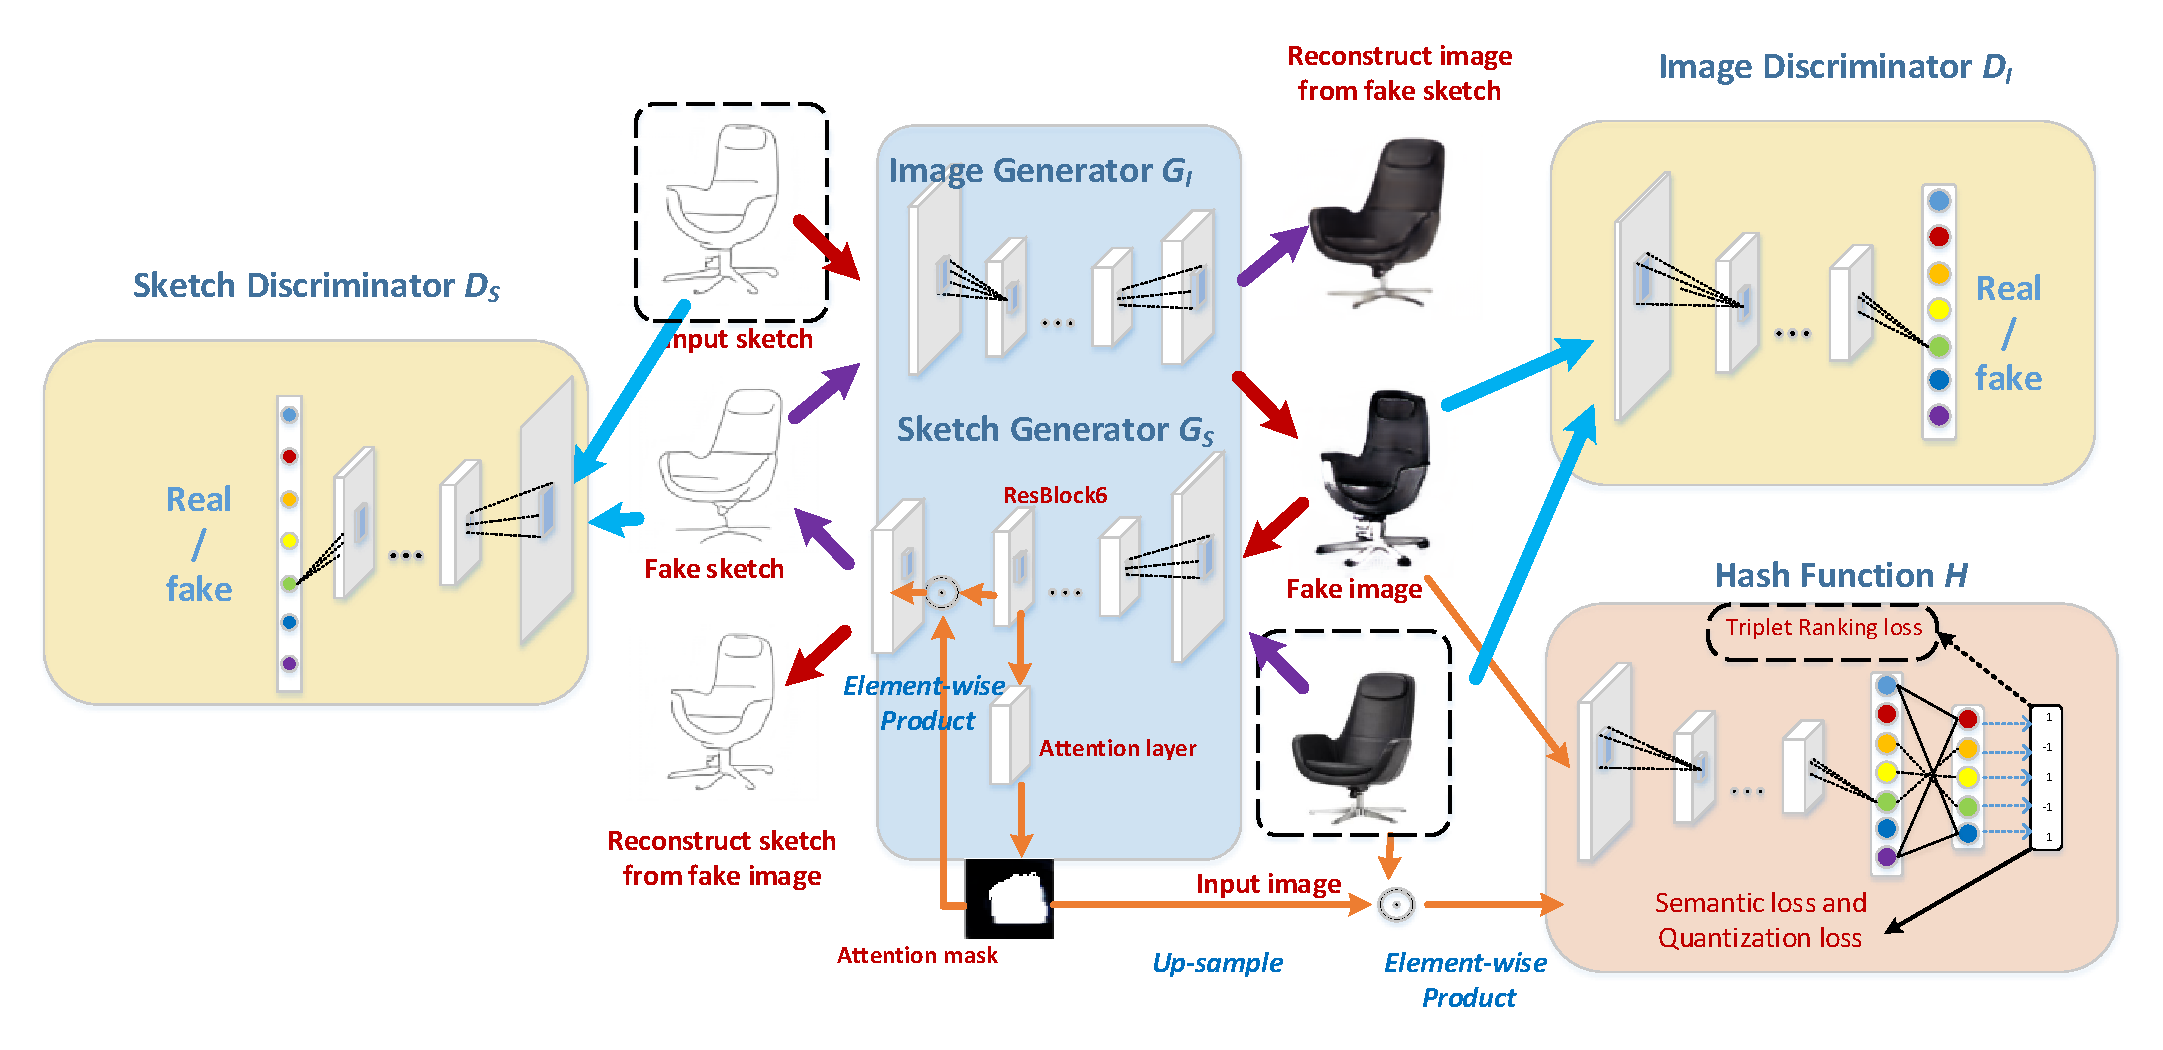
\includegraphics[width = 1\textwidth]{figures/overview2.pdf}
%     \caption{Our deep model for domain-shift and compact binary code learning. On left of the CycleGANs, we fed sketches and images to train a high quility generator $G_I$, which 
%     embeds sketches to images. The top right part is our hash function $H_A$ with the inputs of real images and fake images. And the semantic loss (triplet ranking loss for fine-grained retrieval) and quantization loss are calculated here, which enables the $H_A$ net generates high quaility binary codes.}
%     \label{fig:overview}
% \end{figure*}



\section{Generative Domain-migration Hash}
\subsection{Preliminary}
Given $n_1$ training images $I= \left \{ I_i \right \}^{n_1}_{i=1}$ and $n_2$ training sketches $S= \left \{ S_i \right \}^{n_2}_{i=1}$, the label vectors (row vectors) for all the training instances are $Y^I = \left \{ \mathbf{y}^I_i \right \}^{n_1}_{i=1}\in \{0, 1\}^{n_1\times c}$ and $Y^S = \left \{ \mathbf{y}^S_i \right \}^{n_2}_{i=1}\in \{0,1\}^{n_2\times c}$, respectively, where $\mathbf{y}^I_i$ and $\mathbf{y}^S_i$ are one-hot vectors and $c$ is the number of classes.
We aim to learn the migration from sketches to natural images, and simultaneously learn the hashing function $\mathbf{H} : \{I, I_{fake} \} \rightarrow \left \{ -1,+1 \right \}^K$, such that the semantic consistency can be preserved between the extracted hashing codes of both authentic and generated natural images.

%Our goal is to first generate fake images $I_{fake}$ from sketches $S$, and then learn hashing models $\mathbf{H} : \{I, I_{fake} \} \rightarrow \left \{ -1,+1 \right \}^K$ to map authentic images and fake images to $K$-bit hash codes.
% * <jgg_jingyizhang@foxmail.com> 2018-03-08T12:09:42.581Z:
%
% ^.
%\vspace{-5mm}



\subsection{Network Architecture}
To serve the above purposes, we simultaneously optimize a pair of generative and discriminative networks and a hashing network.
%As mentioned above, since images and sketches typically have tremendous domain gap and various distributions, it is difficult to connect them directly from such cross-domain retrieval task. To bridge this gap, we propose domain-migration networks for mutually conversion between sketches and images, which can effectively narrow the domain gap and better preserve the underlying cross-model similarity in the data structure. In this way, it will output a domain invariant binary representation for retrieval. 
%The general framework of our proposed method is shown in Fig. \ref{fig:overview}. 
 
\noindent\textbf{Generative networks:} Let $G_I$ and $G_S$ be two parallel generative CNNs for migrating sketches to the natural images and vice versa: $G_I : S \rightarrow I$ and $G_S : I \rightarrow S$. The detailed architectures of CNNs are illustrated in Table \ref{table:network}. Considering natural images contain much more information than their sketch counterparts, migrating sketches to natural images is essentially an upsampling process and potentially requires more parameters. 

In order to suppress the background information and guide the learning process to concentrate on the most representative regions, we integrate an attention module \cite{song2017deep,abs-1711-09347} in $G_S$. The attention module contains a convolutional layer with 1$\times$1 kernel size, where a softmax function with a threshold is applied to the output for obtaining a binary attention mask. Element-wise $\odot$ multiplication can be performed between the binary attention mask and the feature map from ResBlocks.

%In addition, since the background of real images is too complex, we try to add an attention layer \cite{song2017deep,abs-1711-09347} to $G_I$ to extract the most important part of the corresponding image. We first feed the image feature maps after ResBlocks into one layer neural network, i.e., a convolutional layer with 1$\times$1 kernel size. Then a softmax function and a threshold function will generate the attention distribution over the regions.
%The output of the threshold function is a 0-1 binary mask. The regions with the value 1 are regarded as the foregrounds or the regions that are attend to, while other regions are regarded as background regions.
%Note that once the $mask$ is generated, it will be up-sampled and fused with the real image as $I \odot mask$, where $\odot$ is the element-wise multiplication. Then $I \odot mask$ will be as inputs of $G_S$, $D_I$ and $\mathbf{H}$. We only add the attention layer to $G_I$ and the attention $mask$ is only fused with the real image. Through this operation, we can avoid the complex background of images disturbing the mapping function $G_S : I \rightarrow S$ to some extent and make the inputs of the hash network robuster. The detailed parameters are listed in Table \ref{table:network}.
 
\noindent\textbf{Discriminative networks:} Along with two generators, two discriminative networks are correspondingly integrated in GDH, where $D_I$ aims to distinguish the images with its mask ($I \odot mask$) and the generated images $G_I\left(S\right)$, and $D_S$ aims to distinguish the real sketches $S$ and the generated sketches $G_S\left(I\right)$. 

\noindent\textbf{Hashing network:} The hashing network $\mathbf{H}$ aims to generate binary hashing codes of both real images $I$ and generated images $G_I\left(S\right)$, and can be trained based on both real image  with its mask ($I \odot mask$) and generated image $G_I\left(S\right)$ from the domain-migration network. The hashing network $\mathbf{H}$ is modified from the 18-layer Deep Residual Network (Resnet) \cite{HeZRS16} by replacing the softmax layer with a fully-connected layer with a binary constraint on the values, where the dimension of the fully-connected layer equals to the length of the hashing codes. 

%In the shared-weight hashing network $\mathbf{H}$, a standard 18-layer Deep Residual Network (Resnet) \cite{HeZRS16} is used to embed images and fake images into binary codes. There are two input branches, where the first one is the real image  with its mask ($I \odot mask$) branch , while the other is the fake image $\left(G_I\left(S\right)\right)$ branch. For binary code learning, we replace the last layer of the softmax classifier in the original ResNet18 with a new fully-connected hash layer. For category-level retrieval, the loss is calculated by this layer. For fine-grained retrieval, we add the triplet ranking loss additionally.


We denote the parameters of the shared-weight hashing network as $\bm{\theta}_H$. For natural images and sketches, we formulate the deep hash function (\emph{i.e., the Hashing network} ) as $\mathbf{B}^I = \sgn ( \mathbf{H} ( I \odot mask;\bm{\theta}_H)) \in \{0, 1\}^{n_1 \times K}$ and $\mathbf{B}^S =\sgn ( \mathbf{H} ( G_I ( S);\bm{\theta}_H)) \in \{0, 1\}^{n_2 \times K}$, respectively,
where $\sgn(\cdot)$ is the sign function. Note that we use the row vector of the output for the convenience of computation. In the following section, we will introduce the deep generative hashing objective of joint learning of binary codes and hash functions.


\begin{table}
\newcommand{\tabincell}[2]{\begin{tabular}{@{}#1@{}}#2\end{tabular}}
\caption{Network architecture of the generative domain-migration network.}
\begin{center}
\resizebox{0.99\textwidth}{!}{
\begin{tabular}{c|c|c|c|c|c||c|c|c|c|c|c}
\hline
\textbf{Net} & \textbf{Layer} & \textbf{Kernel Size} & \textbf{Stride} & \textbf{Pad}& \textbf{Output} &\textbf{Net} & \textbf{Layer} & \textbf{Kernel Size} & \textbf{Stride} & \textbf{Pad}& \textbf{Output}\\
\hline
\hline
\multirow{10}{*}{\tabincell{c}{\textbf{$G_S$-Net}\\}}
&input &- &- &- &3$\times$256$\times$256 &\multirow{10}{*}{\tabincell{c}{\textbf{$G_I$-Net}\\}}
&input &- &- &- &3$\times$256$\times$256 \\\cline{2-6} \cline{8-12} 
&\emph{conv1 BN} &3$\times$3 &1 &1 &32$\times$256$\times$256 &&\emph{conv1 BN} &3$\times$3 &1 &1 &32$\times$256$\times$256 \\
&\emph{conv2 BN} &3$\times$3 &1 &1 &32$\times$256$\times$256 &&\emph{conv1 BN} &3$\times$3 &1 &1 &32$\times$256$\times$256 \\
&\emph{conv3 BN} &4$\times$4 &2 &1 &64$\times$128$\times$128 &&\emph{conv2 BN} &4$\times$4 &2 &1 &64$\times$128$\times$128 \\
&\emph{conv4 BN} &4$\times$4 &2 &1 &128$\times$64$\times$64 &&\emph{conv3 BN} &4$\times$4 &2 &1 &128$\times$64$\times$64 \\\cline{2-6}\cline{8-12}
&\emph{*ResBlock}$\times$6 &3$\times$3&1 &1 &128$\times$64$\times$64&&\emph{*ResBlock}$\times$9 &3$\times$3&1 &1 &128$\times$64$\times$64  \\\cline{2-6}\cline{8-12}
&\emph{attention} &1$\times$1 &1 &0 &1$\times$64$\times$64&&\emph{Deconv4 BN} &4$\times$4 &2 &1 &64$\times$128$\times$128 \\ \cline{2-6}
&\emph{Deconv4 BN} &4$\times$4 &2 &1 &64$\times$128$\times$128 &&\emph{Deconv5 BN} &4$\times$4 &1 &1 &32$\times$253$\times$253 \\
&\emph{Deconv5 BN} &4$\times$4 &2 &1 &32$\times$256$\times$256 &&\emph{Deconv6 BN} &3$\times$3 &1 &1 &3$\times$256$\times$256 \\ \cline{8-12}
&\emph{Deconv6 BN} &3$\times$3 &1 &1 &3$\times$256$\times$256 &&&&&&\\
\hline
\hline
\multirow{7}{*}{\tabincell{c}{\textbf{$D_S$-Net}\\}}
&input &- &- &- &3$\times$256$\times$256 &\multirow{7}{*}{\tabincell{c}{\textbf{$D_I$-Net}\\}}
&input &- &- &- &3$\times$256$\times$256 \\\cline{2-6} \cline{8-12} 
&\emph{conv1 BN} &4$\times$4 &2 &1 &64$\times$128$\times$128 &&\emph{conv1 BN} &4$\times$4 &2 &1 &64$\times$128$\times$128 \\
&\emph{conv2 BN} &4$\times$4 &2 &1 &128$\times$64$\times$64 &&\emph{conv2 BN} &4$\times$4 &2 &1 &128$\times$64$\times$64 \\
&\emph{conv3 BN} &4$\times$4 &2 &1 &256$\times$32$\times$32 &&\emph{conv3 BN } &4$\times$4 &2 &1 &256$\times$32$\times$32 \\
&\emph{conv4 BN} &3$\times$3 &1 &1 &512$\times$32$\times$32 &&\emph{conv4 BN } &3$\times$3 &1 &1 &512$\times$32$\times$32 \\
&\emph{conv5 BN} &3$\times$3 &1 &1 &128$\times$32$\times$32 &&\emph{conv5 BN } &3$\times$3 &1 &1 &128$\times$32$\times$32 \\
\hline


\end{tabular}
}
\scriptsize
The ResBlock is constructed out of two $conv$ layers with $BN$ and a pass-through through the information from previous layers unchanged. The hyper-parameters of the $conv$ layer are: Kernel Size 3$\times$3, Stride 1, Padding 1 and Channels 128. 
\end{center}
\label{table:network}
\vspace{-5ex}
\end{table}

\subsection{Objective Formulation}
\label{sectin:3.3}
There are five losses in our objective function. The adversarial loss and the cycle consistency loss 
guide the learning of the domain-migration network. The semantic and triplet losses preserve the semantic consistency and visual similarity of intra-class instances across domains. The quantization loss and unification constraint can preserve the feature space similarity of pair instances. Detailed discussion of each loss is provided in following paragraphs.

\noindent\textbf{Adversarial and Cycle Consistency Loss:} Our domain-migration networks are composed of four parts: $G_I$, $G_S$, $D_I$ and $D_S$ \cite{ZhuPIE17}.  We denote the parameters of $G_I$, $G_S$, $D_I$ and $D_S$ as $\bm{\theta}_C$. Specifically, $\bm{\theta}_C|_{G_I}$ is the parameter of $G_I$ and so forth. Note that the inputs of domain-migration networks should be image-sketch pairs and usually we have $n_1 \gg n_2$. Thus we reuse the sketches from same category to match the images. Sketches from the same category are randomly repeated and $S$ will be expanded to $\hat{S} =  \{ S_1,\cdots,S_1, S_2 \cdots,S_2, \cdots, S_{n_2},\cdots,S_{n_2}  \}$ to make sure $|\hat{S}| = |I|$.  Suppose the data distributions are $I \sim p_{I}$ and $\hat{S} \sim p_{\hat{S}}$. For the generator $G_I : \hat{S}\rightarrow I$ and its discriminator $D_I$, the adversarial loss can be written as
\begin{equation}\label{eq:equiv1}
\begin{split}
	\min_{\bm{\theta}_C|_{G_I}} \max_{\bm{\theta}_C|_{D_I}} \mathcal{L}_{G}(G_I,D_I,\hat{S},I) & := \mathbf{E}_{I \sim p_{I}}[\log D_I(I \odot mask, \bm{\theta}_C|_{D_I})]\\
	& + \mathbf{E}_{\hat{S} \sim p_{\hat{S}}}[\log(1 - D_I(G_I(\hat{S}, \bm{\theta}_C|_{G_I}), \bm{\theta}_C|_{D_I})],
\end{split}
\end{equation}
where the generator and the discriminator compete in a two-player minimax game: the generator tries to generate images $G_I(\hat{S})$ that look similar to the images from domain $I$ and its corresponding $mask$, while the discriminator tries to distinguish between real images and fake images. The adversarial loss of the other mapping function $G_S : I\rightarrow \hat{S}$ is defined in the similar way. The Cycle Consistency Loss can prevent the learned mapping function $G_I$ and $G_S$ from conflicting against each other, which can be expressed as
\begin{equation}\label{eq:equiv2}
\begin{split}
	\min_{\bm{\theta}_C|_{G_I}, \bm{\theta}_C|_{G_S}}  \mathcal{L}_{cyc}(G_I,G_S)& := \mathbf{E}_{I \sim p_{I}} \| G_S ( G_I ( \hat{S}, \bm{\theta}_C|_{G_I}  ),  \bm{\theta}_C|_{G_S}  )-\hat{S}  \| \\
	&+ \mathbf{E}_{\hat{S} \sim p_{\hat{S}}} \| G_I ( G_S ( I , \bm{\theta}_C|_{G_S} ), \bm{\theta}_C|_{G_I}  )-I \odot mask  \|.
\end{split}
\end{equation}
where $\|\cdot \|$ is the Frobenius norm. The full optimization problem for domain-migration networks is
\begin{equation}\label{eq:equiv3}
 \min_{\substack{\bm{\theta}_C|_{G_I} \\ \bm{\theta}_C|_{G_S}}}  \max_{\substack{\bm{\theta}_C|_{D_I} \\ \bm{\theta}_C|_{D_S}}} \mathcal{L}_{gan} 
:= \mathcal{L}_{G}(G_I,D_I,\hat{S},I) + \mathcal{L}_{G}(G_S,D_S,I,\hat{S}) + \upsilon\mathcal{L}_{cyc}(G_I,G_S).
\end{equation}
We set the balance parameter $\upsilon = 10$ in the experiment according to the previous work \cite{ZhuPIE17}.

\noindent\textbf{Semantic Loss:} %We first define the similarity matrix of $I$ and $S$ as $\mathbf{Y}\in \mathbb{R}^{n\times n}$, in which the element $\mathbf{Y}_{ij}$ denotes the similarity of $\left \{ I_i, I_j \right \}$. We set $\mathbf{Y}_{ij} = 1$ if they have the same label vectors $\mathbf{y}^I_i = \mathbf{y}^I_j$, otherwise $\mathbf{Y}_{ij} = -1$. The similarity of $\left \{ S_i, S_j \right \}$ is the same as $\left \{I_i, I_j \right \}$. 
The label vectors of images and sketches are $Y^I$ and $Y^S$. Inspired by Fast Supervised Discrete Hashing \cite{GuiLSTT18}, we consider the following semantic factorization problem with the projection matrix $\mathbf{D} \in \mathbb{R}^{c\times K}$:
\begin{equation}\label{eq:equiv4}
\begin{split}
	\min_{\mathbf{B}^I, \mathbf{B}^S, \mathbf{D}}\; &\mathcal{L}_{sem} := \left \|  \mathbf{B}^I - Y^I\mathbf{D}\right \|^2 + \left \|  \mathbf{B}^S - Y^S\mathbf{D}\right \|^2 +  \left \|  \mathbf{D}\right \|^2,\\
	\st &\; \mathbf{B}^I  \in\{-1,+1\}^{n_1 \times K}, \mathbf{B}^S  \in\{-1,+1\}^{n_2 \times K}.
\end{split}
\end{equation}
$\mathcal{L}_{sem}$  aims to minimize the distance between the binary codes of the same category, and maximize the distance between the binary codes of different categories.

\noindent\textbf{Quantization Loss:} The quantization loss is introduced to preserve the intrinsic structure of the data, and can be formulated as follows:
\begin{equation}\label{eq:equiv5}
\begin{split}
&\min_{\bm{\theta}_H}\;\mathcal{L}_{q} :=  \left \|  \mathbf{H}\left ( I ;\bm{\theta}_H\right ) -\mathbf{B}^I\right \|^2 +\left \|  \mathbf{H}\left ( G_I\left ( S, \bm{\theta}_C|_{G_I} \right );\bm{\theta}_H  \right ) -\mathbf{B}^S\right \|^2. \\
%&\min_{\bm{\theta}_H}\;\mathcal{L}_{cons2} := \left \|  \mathbf{H}\left ( I ;\bm{\theta}_H\right ) -\mathbf{H}\left (G_I\left ( S \right );\bm{\theta}_H  \right ) \right \|^2 \\
%&\min_{\bm{\theta}_H}\;\mathcal{L}_{reg1} :=  \left \|  \mathbf{H}\left ( I ;\bm{\theta}_H\right ) \mathbf{H}\left ( I ;\bm{\theta}_H\right )^T -K\mathbf{I}\right \|^2 \\
%	&\;\;\;\;\;\;\;\;\;\;\;\;\;\;\;\;\;\;+ \left \|  \mathbf{H}\left ( G_I\left ( S \right );\bm{\theta}_H  \right ) \mathbf{H}\left ( G_I\left ( S \right );\bm{\theta}_H  \right )^T -K\mathbf{I}\right \|^2 \\
%&\min_{\bm{\theta}_H}\;\mathcal{L}_{reg2} := \left \|  \mathbf{H}\left ( I ;\bm{\theta}_H\right ) \right \|^2 +\left \|  \mathbf{H}\left ( G_I\left ( S \right );\bm{\theta}_H  \right ) \right \|^2 \\
\end{split}
\end{equation}

\noindent\textbf{Triplet Ranking Loss:} For the fine-grained retrieval task, we integrate the triplet ranking loss into the objective function for preserving the similarity of paired cross-domain instances within an object category. For a given triplet $\left(S_i,I_i^+,I_i^-\right)$, specifically, each triplet contains a query sketch $S_i$ and a positive image sample $I_i^+$ and a negative image sample $I_i^-$. 
%Moreover, we can regard outputs $\mathbf{H}\left ( G_I\left ( S_i \right );\bm{\theta}_H \right )$ and $\mathbf{H}\left ( I_i;\bm{\theta}_H \right )$ as features which carry meaningful information such as  semantic information, content information and etc. 
%To simplify this problem and narrow the domain gap further, we propose a feature fusion method : using a linear embedding to mix up the two types of features. 
We define the triplet ranking loss function as follow:
\begin{equation}\label{eq:equiv6}
\begin{split}
\min_{\bm{\theta}_H}\;\mathcal{L}_{tri} := &\sum_{i} \max\big( 0, \Delta +\left \| \mathbf{H}\left ( G_I\left ( S_i, \bm{\theta}_C|_{G_I} \right );\bm{\theta}_H \right ) - \mathbf{H}\left ( I_i^+;\bm{\theta}_H \right ) \right \|^2\\
-&\left \|  \mathbf{H}\left ( G_I\left ( S_i, \bm{\theta}_C|_{G_I} \right );\bm{\theta}_H \right ) - \mathbf{H}\left ( I_i^-;\bm{\theta}_H \right )\right \|^2 \big),\\
\end{split}
\end{equation}
where the parameter $\Delta$ represents the margin between the similarities of the outputs of the two pairs $(S_i, I_i^+)$ and $(S_i, I_i^-)$. In other words, the hashing network ensures that the Hamming distance between the outputs of the negative pair $(S_i, I_i^-)$ is larger than the Hamming distance between the outputs of the positive pair $(S_i, I_i^+)$ by at least a  margin of $\Delta$. In this paper, we let $\Delta$ equal to half of the code length (\textit{i.e.}, $\Delta=0.5K$).
%and we will analyze its effectiveness in the experiment.
%We do consider more complex fusion function. However, from the perspective of Occam’s razor, linearity is a good inductive bias since it is one of the simplest possible behaviors[]. And the results are convincing.

\noindent\textbf{Full Objective Function:} We also desire the binary codes of a real natural image and a generated image to be close to each other. Thus, we employ a unification constraint $\mathcal{L}_{c} =  \|  \mathbf{H} ( I ;\bm{\theta}_H ) -\mathbf{H} (G_I ( \hat{S}, \bm{\theta}_C|_{G_I} );\bm{\theta}_H   )  \|^2$ is added to the final objective function which is formulated as follows:
\begin{equation}\label{eq:equiv7}
\begin{split}
&\min_{\mathbf{B^I,B^S, D}, \bm{\theta}_C, \bm{\theta}_H}\;\mathcal{L}_{total} := \mathcal{L}_{gan}+\mathcal{L}_{sem}+ \lambda\mathcal{L}_{tri}+ \alpha\mathcal{L}_{q}+ \beta\mathcal{L}_{c}, \\
%&\;\;\;\;\;\;\;\;\;\;\;\;\;\;\;\;\;\;\;\;\;\;\;\;\;\;\;\;\;\;\;\;+ \alpha\mathcal{L}_{cons1}+ \beta\mathcal{L}_{cons2} \\%+ \gamma\mathcal{L}_{reg1} + \eta\mathcal{L}_{reg2} \\
&\st \; \mathbf{B}^I  \in\{-1,+1\}^{n_1 \times K}, \mathbf{B}^S  \in\{-1,+1\}^{n_2 \times K},\\
\end{split}
\end{equation}
where $\lambda$ is a control parameter, which equals 1 for fine-grained task and equals 0 for semantic-level SBIR only, The hyper-parameters $\alpha$ and $\beta$ control the contributions of the two corresponding terms.


\subsection{Joint Optimization}
Due to the non-convexity of the joint optimization and \textbf{NP}-hardness to output the discrete binary codes, it is infeasible to find the global optimal solution. Inspired by \cite{GuiLSTT18}, we propose an  optimization algorithm  based on alternating iteration and sequentially optimize one variable while the others are fixed. In this way, variables $\mathbf{D}$, $\mathbf{B}^I$, $\mathbf{B}^S$, parameter $\bm{\theta}_C$ of the domain-migration networks, and parameter $\bm{\theta}_H$ of the hash function will be iteratively updated.

\paragraph{$\mathbf{D}$-Step.} By fixing all the variables except $\mathbf{D}$, Eq. \eqref{eq:equiv7} can be simplified as a classic quadratic regression problem:
\begin{equation}\label{eq:equiv8}
\begin{split}
&\min_{\mathbf{D}} \left \|  \mathbf{B}^I - Y^I\mathbf{D}\right \|^2 + \left \|  \mathbf{B}^S - Y^S\mathbf{D}\right \|^2 + \left \|  \mathbf{D}\right \|^2\\
&= \min_{\mathbf{D}} tr\left(\mathbf{D}^{\top} \left({Y^I}^{\top} Y^I+ {Y^S}^{\top} Y^S+\mathbf{I}\right)\mathbf{D}\right)- 2tr\left(\mathbf{D}^{\top} \left( {Y^I}^{\top} \mathbf{B}^I+{Y^S}^{\top}\mathbf{B}^S\right)\right),
\end{split}
\end{equation}
where $\mathbf{I}$ is the identity matrix. Taking the derivative of the above function with respect to $\mathbf{D}$ and setting it to zero, we have the analytical solution to Eq. \eqref{eq:equiv8}:
\begin{equation}\label{eq:equiv9}
\begin{split}
  % temp1 = 2*Sim.t().mm(Sim)+ torch.eye(num_train)
  % temp1 = temp1.inverse()
  % temp1 = temp1.mm(Sim.t())
  % D = temp1.mm((B_I+B_S))
&\mathbf{D} = \left ({Y^I}^{\top} Y^I+ {Y^S}^{\top} Y^S+\mathbf{I}\right )^{-1}\left ({Y^I}^{\top} \mathbf{B}^I+{Y^S}^{\top}\mathbf{B}^S \right).
\end{split}
\end{equation}

\paragraph{$\mathbf{B}^I$-Step.} When all the variables are fixed except $\mathbf{B}^I$, we rewrite Eq. \eqref{eq:equiv7} as
\begin{equation}\label{eq:equiv10}
\min_{\mathbf{B}^I}\; \left \|  \mathbf{B}^I - {Y^I} \mathbf{D}\right \|^2 + \alpha\left \|  \mathbf{H}\left ( I ;\bm{\theta}_H\right ) -\mathbf{B}^I\right \|^2.
\end{equation}
Since $tr\left({\mathbf{B}^I}^{\top} \mathbf{B}^I\right)$ is a constant, Eq. \eqref{eq:equiv10} is equivalent to the following problem:
\begin{equation}\label{eq:equiv11}
\min_{\mathbf{B}^I}\; -tr\left (  {\mathbf{B}^I}^{\top}\left({Y^I} \mathbf{D}+\alpha\mathbf{H}\left ( I ;\bm{\theta}_H\right )\right)\right ).
\end{equation}
For $\mathbf{B}^I  \in\{-1,+1\}^{n_1 \times K} $, $\mathbf{B}^I$ has a closed-form solution as follows:
\begin{equation}\label{eq:equiv12}
\begin{split}
&\mathbf{B}^I = \sgn\left({Y^I}\mathbf{D}+\alpha\mathbf{H}\left( I ;\bm{\theta}_H\right )\right).
\end{split}
\end{equation}
%In this method, the binary codes $\mathbf{B}^I$ can be optimized by a single step, which makes it much faster than the Discrete Cyclic Coordinate descent (DCC) \cite{shen2015supervised}.

\paragraph{$\mathbf{B}^S$-Step.} Considering all the terms related to $\mathbf{B}^S$, it can be learned by a similar formulation as Eq.\eqref{eq:equiv12}:
\begin{equation}\label{eq:equiv13}
\begin{split}
&\mathbf{B}^S = \sgn\left({Y^S}\mathbf{D}+\alpha\mathbf{H}\left ( G_I\left ( S, \bm{\theta}_C|_{G_I} \right );\bm{\theta}_H  \right )\right ).
\end{split}
\end{equation}


\paragraph{$(\bm{\theta}_C ,\bm{\theta}_H)$-Step.} After the optimization for $\mathbf{D}$, $\mathbf{B}^I$ and $\mathbf{B}^S$, we update the network parameters $\bm{\theta}_C$ and $\bm{\theta}_H$ according to the following loss:
\begin{equation}\label{eq:equiv14}
\begin{split}
&\min_{\bm{\theta}_C, \bm{\theta}_H}\;\mathcal{L} := \mathcal{L}_{gan} + \lambda\mathcal{L}_{tri} + \alpha\mathcal{L}_{q}+ \beta\mathcal{L}_{c}. %+ \gamma\mathcal{L}_{reg1} + \eta\mathcal{L}_{reg2} \\
\end{split}
\end{equation} 
We train our networks on $I$ and $\hat{S}$, where the sketch-image pairs are randomly select to compose of the mini-batch, and then backpropagation algorithm with SGD is adopted for optimizing two networks. 
%The inputs of \eqref{eq:equiv1} should be image-sketch pairs and usually we have $n_1 \gg n_2$. Hence, we expand $S$ to $\hat{S}$ to ensure each sketch or natural image has a paired counterpart.
In practice, we use deep learning frameworks (\emph{e.g.}, Pytorch) to achieve all the steps. We iteratively update $\mathbf{D}\rightarrow \mathbf{B}^I \rightarrow \mathbf{B}^S \rightarrow \{\bm{\theta}_C ,\bm{\theta}_H\}$ in each epoch. As such, GDH
can be finally optimized within $L$ epochs, where $20 \leq L \leq 30$ in our experiment.
The algorithm of GDH is illustrated in Algorithm \ref{alg:a1}.

%\vspace{-1ex}
\begin{algorithm}
\small
       \caption{Generative Domain-migration Hash (GDH)}
       \label{alg:GDH}
       \KwIn{Training natural images $I= \left \{ I_i \right \}^{n_1}_{i=1}$ and the corresponding sketches $S= \left \{ S_i\right \}^{n_2}_{i=1}$; the label information $Y^I$ and $Y^S$; the code length $K$; the number of training epochs $L$; the balance parameters $\alpha, \beta, \lambda.$}
       \KwOut{Generative models $G_I$ and $G_S$; deep hash function $\mathbf{H}$.} 
        1: Randomly initialize $\mathbf{B}^I\in\left \{ -1,+1 \right \}^{n_1 \times K}$ and $\mathbf{B}^S \in\left \{ -1,+1 \right \}^{n_2 \times K}$;
        
        2: \textbf{For} $l = 1, 2, \cdots, L$ \textbf{do}

        3: $\;\;$ Update $\mathbf{D}$ according to Eq. \eqref{eq:equiv9};

        4:  $\;\;$ Update $\mathbf{B}^I$ according to Eq. \eqref{eq:equiv12};

        5:  $\;\;$ Update $\mathbf{B}^S$ according to Eq. \eqref{eq:equiv13};

        6:  $\;\;$ Update the network parameters $\bm{\theta}_C$ and $\bm{\theta}_H$ according to Eq. \eqref{eq:equiv14} by training with the $l$-th epoch data;

        7: $\textbf{End}$
        
        8: \textbf{Return} the network parameters $\bm{\theta}_C$ and $\bm{\theta}_H$.
      \label{alg:a1}
\end{algorithm}
%\vspace{-1ex}


Once GDH model is learned, for a given query sketch $s_q$, we can infer its binary code $\mathbf{b}^{s_q} = \sgn\left (\mathbf{H}\left ( G_I\left ( S_q, \bm{\theta}_C|_{G_I} \right );\bm{\theta}_H  \right )\right)$ through the $G_I$ network and the hash network $\mathbf{H}$. For the image gallery, the hash codes $\mathbf{b}^I = \sgn\left(\mathbf{H}\left( I \odot mask ;\bm{\theta}_H\right )\right)$ of each image is computed through the hash network, where $mask$ can be easily obtained by $G_S\left(I;\bm{\theta}_C|_{G_S}\right)$. Note that fake images generated by $G_I\left ( S_q, \bm{\theta}_C|_{G_I} \right )$ are non-background and thus they don't need multiply $mask$ before feed into the hashing network.

\section{Experiments and Results}
In the experiment section, we aim to address the following
three questions:
\begin{itemize}
\vspace{-1ex}
\item How does GDH perform as compared to other state-of-the-art binary or real-valued methods for category-level SBIR?
\item How does GDH perform as compared to other state-of-the-art real-valued methods for fine-grained SBIR?
\item How does each component or constraint contribute to the overall performance of GDH?
\vspace{-1ex}
\end{itemize}

\subsection{Datasets and Settings}
\vspace{-1ex}
\subsubsection{Category-level Retrieval.} GDH is evaluated on two largest SBIR datasets: Sketchy \cite{SangkloyBHH16} and TU-Berlin \cite{EitzHA12} Extension. The Sketchy database contains 125 categories with 75,471 sketches of 12,500 object images. We additionally utilize another 60,502 natural images \cite{LiuSSLS17} collected from ImageNet \cite{deng2009imagenet}. Hence, the whole image database contains 73,002 images in total. 
TU-Berlin is a sketch dataset with 250 object categories, where each category contains 80 sketches. An additional 204,489 natural images associated with TU-Berlin provided by \cite{0008LZRWC16} are used to construct the image database. Similar to previous hashing experiments \cite{LiuSSLS17}, 50 and 10 sketches are respectively selected as the query sets for TU-Berlin and Sketchy, where the remaining are used as the gallery for training. 

%\textbf{Baseline and Evaluation Setup} 
We compare GDH with 8 existing category-level SBIR methods, including 4 hand-crafted methods: LSK \cite{SaavedraB15}, SEHLO \cite{Saavedra14}, GF-HOG \cite{hu2010} and HOG \cite{dalal2005}; and 4 deep learning based methods: 3D shape \cite{WangKL15}, Sketch-a-Net (SaN) \cite{sketchanet}, GN Triplet \cite{SangkloyBHH16} and Siamese CNN \cite{QiSZL16}. Furthermore, we also compare GDH with 7 state-of-the-art cross-modality hashing methods: Collective Matrix Factorization Hashing (CMFH) \cite{DingGZ14}, Cross-Model Semi-Supervised Hashing (CMSSH) \cite{BronsteinBMP10},
Cross-View Hashing(CVH) \cite{KumarU11}, Semantic Correlation Maximization (SCMSeq and SCM-Orth) \cite{ZhangL14}, Semantics-Preserving Hashing(SePH) \cite{LinDH015}, Deep Cross-Modality Hashing (DCMH) \cite{JiangL17} and Deep Sketch Hash (DSH) \cite{LiuSSLS17}. Finally, we also compare our method to other four cross-view feature embedding
methods: CCA \cite{ViaSP05}, PLSR \cite{LiuMHCZ18}, XQDA \cite{LiaoHZL15} and CVFL \cite{XiePX14}. The implementation details and experimental results of above methods are reported in \cite{LiuSSLS17}.

We use the Adam solver \cite{KingmaB14} with a batch size of 32. 
Our balance parameters are set to $\alpha=10^{-5}, \beta=10^{-5}$ and $\lambda=0$ for both datasets.
%\gamma=10^{-5}, \eta=10^{-5}, 
All networks are trained with an initial learning rate $lr=0.0002$. After 25 epochs, we decrease the learning rate of the hashing network $lr\rightarrow 0.1lr$ and terminate the optimization after 30 epochs for both datasets. Our method is implemented by Pytorch with
dual 1080Ti GPUs and an i7-4790K CPU.


\begin{table*}[t]
%\vspace{-2ex}
\center
\newcommand{\tabincell}[2]{\begin{tabular}{@{}#1@{}}#2\end{tabular}}
\caption{Comparison with previous SBIR methods w.r.t. MAP, retrieval time per query ($\mathrm{s}$) and memory cost ($\mathrm{MB}$) on on TU-Berlin Extension and Sketchy.}
\resizebox{0.99\textwidth}{!}{
\begin{tabular}{c|c||c|c|c||c|c|c}
\hline
\multirow{3}{*}{\textbf{Methods}} &\multirow{3}{*}{\textbf{Dimension}}  &\multicolumn{3}{c||}{\textbf{TU-Berlin} \textbf{Extension}}&\multicolumn{3}{c}{\textbf{Sketchy}} \\
\cline{3-8}
& & \textbf{MAP} & \textbf{\tabincell{c}{Retrieval time\\ per query ($\mathrm{s}$)}} & \tabincell{c}{\textbf{Memory cost ($\mathrm{MB}$)}\\(204,489 images)}&\textbf{MAP} &\textbf{\tabincell{c}{Retrieval time\\ per query  ($\mathrm{s}$)}}  & \tabincell{c}{\textbf{Memory cost ($\mathrm{MB}$)}\\(73,002 images)}\\
\hline
HOG \cite{dalal2005} &1296 &0.091  &1.43  &$2.02\times10^3$  &0.115  & 0.53 &$7.22\times10^2$ \\
GF-HOG \cite{hu2010} &3500 &0.119  & 4.13  &$5.46\times10^3$ &0.157 & 1.41 &$1.95\times10^3$ \\
SHELO \cite{Saavedra14} &1296 & 0.123 &1.44  & $2.02\times10^3$  &0.182 &0.50 &$7.22\times10^2$ \\
LKS \cite{SaavedraB15}&1350 &0.157 &0.204  &$2.11\times10^3$   &0.190  &0.56 &$7.52\times10^2$ \\
\hline
Siamese CNN \cite{QiSZL16} &64 &0.322  &  7.70$\times 10^{-2}$  &99.8  &0.481  &2.76$\times 10^{-2}$ &35.4 \\
SaN \cite{sketchanet} &512 &0.154  & 0.53  &$7.98\times10^2$  &0.208 & 0.21 &$2.85\times10^2$ \\
GN Triplet$^{*}$  \cite{SangkloyBHH16} &1024 &0.187  &1.02  &$1.60\times10^3$   &0.529  & 0.41 &$5.70\times10^2$  \\
3D shape$^{*}$ \cite{WangKL15} &64  &0.072&7.53$\times 10^{-2}$  &99.8 &0.084   & 2.64 $\times 10^{-2}$&35.6 \\
\hline
\tabincell{c}{Siamese-AlexNet} &4096 &0.367  &5.35   &$6.39\times10^3$  &0.518  & 1.68 &$2.28\times10^3$ \\
\hline
\tabincell{c}{Triplet-AlexNet}&4096 &0.448  &5.35  &$6.39\times10^3$ &0.573 & 1.68  $\mathrm{s}$&$2.28\times10^3$ \\
\hline
\hline
\multirow{3}{*}{\textbf{\tabincell{c}{GDH\\(Proposed)}}}  &32 (bits)&0.563  &5.57$\times 10^{-4}$   &0.78 &0.724  &2.55$\times 10^{-4}$  &0.28 \\
\cline{2-8}
&64 (bits)&\textbf{0.690}  &7.03$\times 10^{-4}$  &1.56  &\textbf{0.810}  &2.82$\times 10^{-4}$  &0.56 \\
\cline{2-8}
&128 (bits)&0.659&1.05$\times 10^{-3}$  &3.12  &0.784  & 3.53$\times 10^{-4}$ &1.11 \\
\hline
\end{tabular}
}\scriptsize
\\``$\ast$'' denotes that we directly use the public models provided by the original papers without any fine-tuning on the TU-Berlin Extension and Sketchy datasets.
\label{table:t1}
\vspace{-2ex}
\end{table*}

%\textbf{Fine-grained Retrieval}
\vspace{-2ex}
\subsubsection{Fine-grained Retrieval.} We conduct experiments of GDH on the QMUL-Shoes and QMUL-Chairs datasets \cite{Yu2016shoes}. %\textbf{Sketchy} database is for fine-grained task, which contains 125 categories with 75,471 sketches of 12,500 objects. 
The two datasets are  fine-grained instance-level SBIR datasets which contain 419 shoes sketch-photo pairs and 297 chairs sketch-photo pairs, respectively.

We compare our proposed GDH method with several fine-grained methods including 2 hand-crafted methods: 
HOG+BoW+RankSVM \cite{LiHSG15} and Dense HOG+RankSVM \cite{Yu2016shoes}, 
and 3 deep feature baselines: Improved Sketch-a-Net (ISN) \cite{sketchanet}, 
3D shape (3DS) \cite{WangKL15} and Triplet Sketch-a-Net (TSN) \cite{Yu2016shoes}. 
All of these algorithms are real-valued methods.
%For \textbf{sketchy} dataset, following the [The Sketchy Database], we compare our binary method with several real value method: \textbf{GN Triplet},
%\textbf{GN Siamese} and \textbf{AN Siamese}
It is noteworthy that the networks in TSN \cite{Yu2016shoes} are heavily pre-trained and the data have been processed by complex augmentation. However, to emphasize the ability of our domain-migration model, data augmentation is not included in our experiment. 

Note that, QMUL-Shoes and QMUL-Chairs are unique fine-grained datasets, in which only contains one category for each of them. Therefore, it is unnecessary to optimize the semantic loss in Eq. \eqref{eq:equiv7}.  To better fit the task of fine-grained retrieval, we skip the first five steps in Algorithm~\ref{alg:a1} and directly update the parameters of $\bm{\theta}_C$ and $\bm{\theta}_H$. Our balance parameters are set to %$ \gamma=10^{-5}, \eta=10^{-5}, \lambda=1$
$ \lambda=1$.
The implementation details are the same as the settings for category-level retrieval, except that the batch size is 64 and the optimization
%All networks are trained with an intial learining rate $lr=0.002$. And terminate the optimization after 10 epochs.% For Sketchy dataset, the experiment settings are similar to category-level retrieval experiments excepts we set $\lambda=1.$
will be terminated after 200 epochs.





\subsection{Results and Discussions}
\vspace{-1ex}
\subsubsection{Comparison with Category-level SBIR Baselines.} We compare our GDH method with the 10 baseline methods in terms of Mean Average Precision (MAP), retrieval time and memory cost on two datasets. The code lengths of outputs are 32, 64 and 128 bits.  As reported in Table~\ref{table:t1}, GDH consistently achieves the best performance with much faster query time and much lower memory cost compared to other SBIR methods on both datasets. Also, GDH largely improves the state-of-the-art performance of Triplet-AlexNet by 24.2\% and 23.7\% on the TU-Berlin and Sketchy datasets, respectively. The performance of 128 bits is lower than the performance of 64 bits can be explained with the quantization error accumulation \cite{shen2015supervised}. We also notice that the performance of compared methods on both datasets is much lower than reported in previous papers\cite{WangKL15,Yu2016shoes}. The reason is that the data they previously used are all well-aligned with perfect background removal and the edge of objects can almost fit the sketches. Meanwhile, our experiments adopt realistic images with complicated background, which are greatly different from sketches.

%2) The performance of deep methods is much higher than it of hand-crafted methods since the features that deep architecture extracts are much better than the hand-crafted features. (3) The results on sketchy dataset are higher than those on TU-Berlin Extension because the data in sketchy dataset contains fewer categories and is relatively simpler.(4) Among the compared method, we notice that the performance on TU-Berlin Extension and  sketchy dataset is much lower than these reported by previous papers. This is because the data they previously used is all well-aligned with perfect background removal. And the edge of images can almost fit the sketches. However, the data we used is real natural images with complex background and there is a huge gap between image domain and sketch domain. (5) Our GDH is much faster with much lower memory cost compared to  other SBIR method during retrieval.




\begin{table*}[t]
%\vspace{-2ex}
\begin{center}
%\tiny
\newcommand{\tabincell}[2]{\begin{tabular}{@{}#1@{}}#2\end{tabular}}
\caption{MAP comparison with different cross-modality retrieval methods for category-level SBIR on TU-Berlin Extension and Sketchy.}
\resizebox{0.8\textwidth}{!}{
\begin{tabular}{c|c|c|c|c|c|c|c}
  \hline
  \multicolumn{2}{c|}{\multirow{2}{*}{\textbf{Method}}} &\multicolumn{3}{c|}{\textbf{TU-Berlin} \textbf{Extension}} & \multicolumn{3}{c}{\textbf{Sketchy}}\\
\cline{3-8}
  %\multicolumn{2}{|c||}{} &\multicolumn{3}{c||}{\bf MAP}  & \multicolumn{3}{c|}{\bf MAP}  \\
  \cline{3-8}
  \multicolumn{2}{c|}{} &32 bits & 64 bits & 128 bits   & 32 bits & 64 bits & 128 bits \\
  \hline
  \multirow{6}{*}{\tabincell{c}{Cross-Modality\\ Hashing Methods\\(binary codes)}}
  &CMFH \cite{DingGZ14} &0.149 &0.202 &0.180  &0.320 &0.490 &0.190 \\
  &CMSSH  \cite{BronsteinBMP10}  &0.121 &0.183 &0.175  &0.206 &0.211 &0.211 \\
  &SCM-Seq \cite{ZhangL14}  &0.211 &0.276 &0.332  &0.306 &0.417&0.671 \\
  &SCM-Orth \cite{ZhangL14}&0.217 &0.301 &0.263  &0.346 &0.536 &0.616 \\
  &CVH  \cite{KumarU11}&0.214 &0.294 &0.318  &0.325 &0.525 &0.624 \\
 &SePH  \cite{LinDH015}  &0.198 &0.270 &0.282  &0.534 &0.607 &0.640 \\
  &DCMH \cite{JiangL17} &0.274 &0.382 &0.425  &0.560 &0.622 &0.656 \\
  &DSH \cite{LiuSSLS17} &0.358 &0.521 &0.570  &0.653 &0.711 &0.783 \\
  
  \hline
  \multirow{4}{*}{\tabincell{c}{Cross-View Feature \\ Learning Methods\\(real-valued vectors)}}
  &CCA \cite{ViaSP05} &0.276 &0.366 &0.365  &0.361 &0.555 &0.705\\
  &XQDA \cite{LiuMHCZ18} &0.191 &0.197 &0.201  &0.460 &0.557 &0.550 \\
 \cline{3-8}
&PLSR \cite{LiaoHZL15} &\multicolumn{3}{c|}{0.141 (4096-d)}  &\multicolumn{3}{c}{0.462 (4096-d)} \\
  &CVFL \cite{XiePX14} &\multicolumn{3}{c|}{0.289 (4096-d)}  &\multicolumn{3}{c}{0.675 (4096-d)}  \\
  \hline
\textbf{Proposed}& \textbf{GDH}  &\textbf{0.563} &\textbf{0.690}&\textbf{0.651}  &\textbf{0.724} &\textbf{0.811} & \textbf{0.784}\\
   \hline
  \end{tabular}

  }
\label{table:t2}
\scriptsize \\
For end-to-end deep methods, raw natural images and sketches are used.  For others, 4096-d AlexNet \emph{fc7} image features and 512-d SaN \emph{fc7} sketch features are used. PLSR and CVFL are both based on reconstructing partial data to approximate full data, so the dimensions are fixed to 4096-d.
\vspace{-6ex}
\end{center}
\end{table*}




\vspace{-2ex}
\subsubsection{Comparison with Cross-modality Hashing.} In Table~\ref{table:t2}, we compare our GDH method with cross-modality hashing/feature learning methods with 32, 64 and 128 bits binary codes. We use the learned deep features as the inputs for non-end-to-end learning methods for a fair comparison with GDH. GDH achieves the best performance compared to all the cross-modality baselines on both datasets. Specifically, GDH can outperform  the best-performing hashing-based SBIR method DSH \cite{LiuSSLS17}by 20.5\%/7.1\%, 16.9\%/10\% and
8.1\%/0.1\% at different code lengths on both datasets, respectively. In addition, we illustrate the t-SNE visualization in Fig. \ref{fig:tsne-figure} on the Sketchy dataset, which shows the hashing codes of query sketches and the image gallery share common distributions in the embedded space.



\begin{figure*}[t]
 \vspace{-2ex}
    \centering
    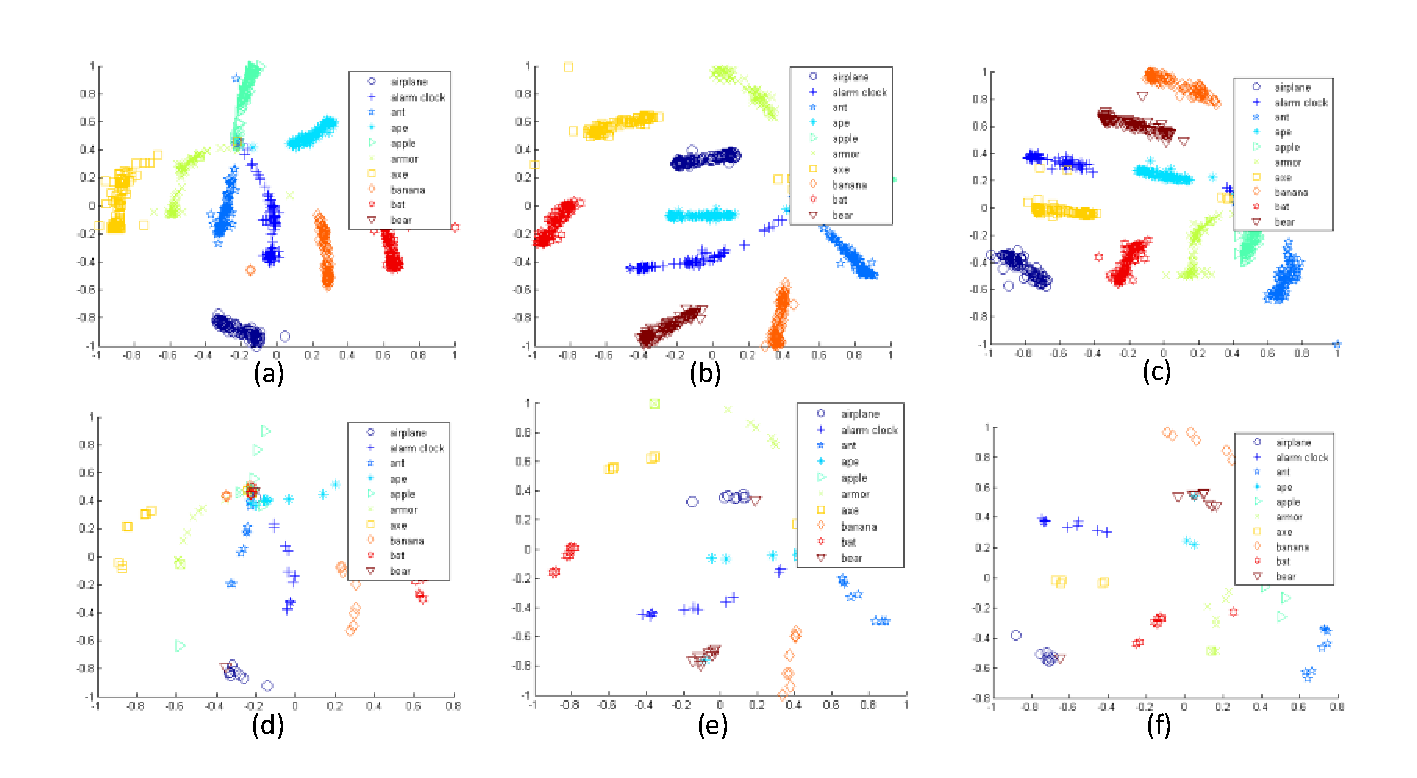
\includegraphics[width = 0.99\textwidth]{figures/tsne.pdf}
    \vspace{-4ex}
    \caption{t-SNE visualization of GDH for 10 representative categories in the Sketchy dataset: (a-c) binary codes of images at 32, 64 and 128 bits; (d-f) binary codes of sketches at 32, 64 and 128 bits. The embedded hash codes of both image and sketch domains share the same distribution and discriminative ability.}
    \label{fig:tsne-figure}
    %\vspace{-2ex}
\end{figure*}




\begin{table*}[t]
%\tiny
\begin{center}

%\footnotesize
\newcommand{\tabincell}[2]{\begin{tabular}{@{}#1@{}}#2\end{tabular}}
\caption{Accuracy comparison with different real-valued methods for fine-grained SBIR on QMUL-shoes and QMUL-chairs.}
\resizebox{0.99\textwidth}{!}{
\begin{tabular}{c|c|c|c|c|c}
  \hline
  \multicolumn{2}{c|}{\multirow{1}{*}{\textbf{Methods}}} &\multicolumn{1}{c|}{\textbf{QMUL-shoes.acc@1}}  &\multicolumn{1}{c|}{\textbf{QMUL-shoes.acc@10}} &\multicolumn{1}{c|}{\textbf{QMUL-chairs.@1}}&\multicolumn{1}{c}{\textbf{QMUL-chairs.@10}}\\
\cline{1-5}
  \hline
  \hline
  \multirow{6}{*}{\tabincell{c}{Real-valued\\ vectors}}
  &BoW-HOG + rankSVM \cite{LiHSG15}  &0.174 &0.678 &0.289 &0.670\\
  &Dense-HOG + rankSVM \cite{Yu2016shoes}   &0.244 &0.652&0.526 &0.938 \\
  &ISN Deep + rankSVM \cite{sketchanet}   &0.200 &0.626 &0.474 &0.825\\
  &3DS Deep + rankSVM \cite{WangKL15}   &0.052 &0.217 &0.061 &0.268\\
  &TSN without data aug. \cite{Yu2016shoes}&0.330 &0.817 &0.644 &0.956 \\
  &TSN with data aug. \cite{Yu2016shoes} &0.391 &0.878 &0.691 & 0.979\\
  \hline
  \hline
  \multirow{3}{*}{\tabincell{c}{ Binary codes}}
 &GDH @ 32-bit &0.286 &0.720 &0.392 & 0.876\\
 &GDH @ 64-bit &0.323 &0.783 &0.556 & 0.959\\
 & GDH @ 128-bit &0.357 &0.843 &0.671 & 0.990\\
  \hline
  \end{tabular}
  }
\label{table:t3}
\scriptsize
To emphasize the ability of our domain-migration model, data augmentation \cite{Yu2016shoes} is not included.
Even so, our binary results are competitive and promising compared to other real-valued methods.
\end{center}
\vspace{-4ex}
\end{table*}

\vspace{-1ex}
\subsubsection{Comparison for Fine-grained SBIR.}
In Table \ref{table:t3}, we report the top-1 and top-10 accuracies of GDH over other five methods on the Shoes and Chairs datasets for fine-grained SBIR. Compared to the state-of-the-art real-valued TSN (without data augmentation), the 128-bit GDH achieves 2.7\%/2.7\% and 2.6\%/3.4\% improvements in terms of top-1 and top-10 accuracies on both the Shoes and Chairs datasets respectively. Specifically, the top-10 accuracy on the Chairs dataset reaches 99\%, which is even higher than the performance of TSN with data augmentation. 

\textbf{Remark.} For fine-grained SBIR, despite binary hashing codes are used, comparable or even improved performance over the real-valued state-of-the-art methods can be observed in Table. \ref{table:t3}. On the other side, the binary codes in GDH allow much reduced memory costs and retrieval time than the real-valued approaches. However, GDH generally shows degraded performance on the fine-grained SBIR when comparing to its performance on category-level SBIR. Our explanation towards such a phenomenon is that the geometrical morphology and detailed instance-level characteristic within a category can be much more difficult to capture with binary hashing codes than the inter-category discrepancies. In Fig. \ref{fig:finegrained-figure}, some examples based on the retrieval results of GDH are illustrated. More illustrations can be found in the \textbf{Supplementary Material}.



\begin{figure*}[t]
    \centering
    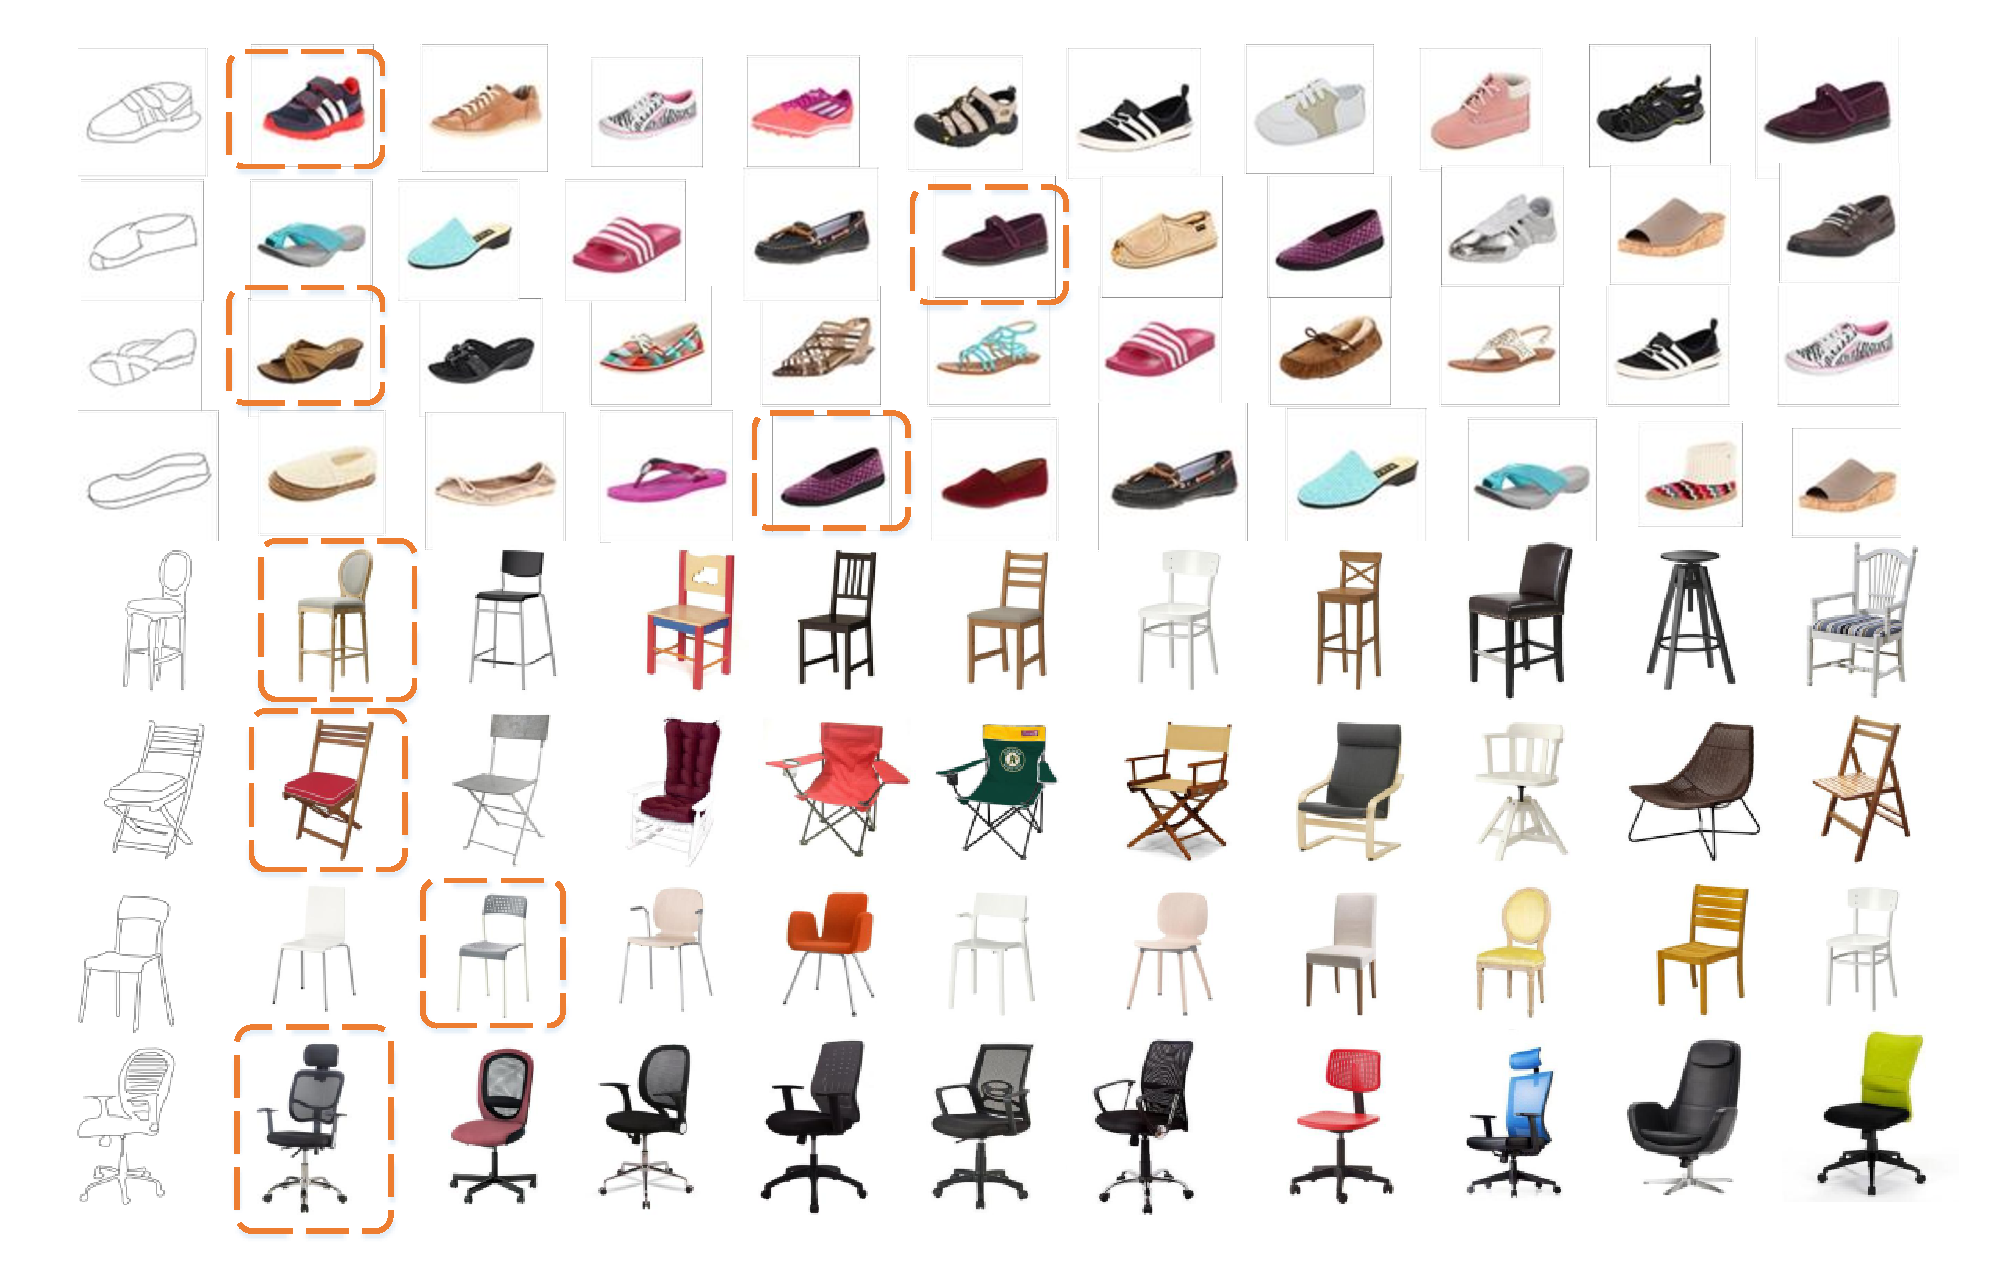
\includegraphics[width = 0.9\textwidth]{figures/shoes_results1.pdf}
    \vspace{-2ex}
    \caption{Example query sketches with their top-10 retrieval accuracies on the Sketchy dataset by using 128-bit GDH codes. Orange boxes indicate the groundtruth results.}
    \label{fig:finegrained-figure}
    \vspace{-3ex}
\end{figure*}


% \begin{table*}[ht]
% %\tiny
% \begin{center}

% %\footnotesize
% \newcommand{\tabincell}[2]{\begin{tabular}{@{}#1@{}}#2\end{tabular}}
% \caption{Comparative results for Fine-grained SBIR. }
% \resizebox{0.999\textwidth}{!}{
% \begin{tabular}{c|cc}
%   \hline
%   \multicolumn{1}{c|}{\multirow{1}{*}{\textbf{Shoe Datas}}} &\multicolumn{1}{c}{\textbf{acc.@1}} & \multicolumn{1}{c}{\textbf{acc.@10}}\\
% \cline{1-3}
%   \hline
%   \hline
%   BoW-HOG + rankSVM  &0.174 &0.678 \\
%   Dense-HOG + rankSVM  &0.244 &0.652  \\
%   ISN Deep + rankSVM  &0.200 &0.626  \\
%   3DS Deep + rankSVM&0.052 &0.217  \\
%   Sketch me that shoe without data aug &0.330 &0.817  \\
%    \hline
% %Our model GDH 32bit &0.562 &0.948\\
% %Our model GDH 64bit &0.748 &\textbf{1.00}\\
% Our model GDH 128bit(binary) &\textbf{0.347} &\textbf{0.846}\\
%  Sketch me that shoe with data aug &0.391 &0.878  \\
%   \hline\hline
%   \end{tabular}
%   }
% \label{table:t3}
% \scriptsize
% \vspace{-4ex}
% \end{center}
% \end{table*}


% \begin{table*}[t]
% \begin{center}
% %\footnotesize
% \newcommand{\tabincell}[2]{\begin{tabular}{@{}#1@{}}#2\end{tabular}}
% \caption{ Comparison with different continuous value methods for fine-grained SBIR. }
% \resizebox{0.999\textwidth}{!}{
% \begin{tabular}{|c|c||c|c||c|c|}
%   \hline
%   \multicolumn{2}{|c||}{\multirow{2}{*}{\textbf{Method}}} &\multicolumn{2}{c||}{\textbf{Shoes}} & \multicolumn{2}{c|}{\textbf{Chairs}}\\
% \cline{3-6}
%   \multicolumn{2}{|c||}{} &\multicolumn{2}{c||}{\bf acc.}  & \multicolumn{2}{c|}{\bf acc.}  \\
%   \cline{3-6}
%   \multicolumn{2}{|c||}{} & @ 1 & @ 10   & @ 1  & @ 10 \\
%   \hline
%   \hline
%   \multirow{6}{*}{\tabincell{c}{Cross-Modality\\Continuous value Methods\\ }}
%   &BoW-HOG + rankSVM \cite{LiHSG15}  &0.174 &0.678 &0.289 &0.670\\
%   &Dense-HOG + rankSVM \cite{Yu2016shoes}   &0.244 &0.652&0.526 &0.938 \\
%   &ISN Deep + rankSVM \cite{sketchanet}   &0.200 &0.626 &0.474 &0.825\\
%   &3DS Deep + rankSVM \cite{WangKL15}   &0.052 &0.217 &0.061 &0.268\\
%   &MTL without data aug. \cite{Yu2016shoes}&0.330 &0.817 &0.644 &0.956 \\
%   &MTL with data aug \cite{Yu2016shoes} &0.391 &0.878 &0.691 & 0.979\\
%   \hline
%   \hline
%   Our proposed 128 bits binary method &GDH &0.357 &0.843 &0.671 & 0.990\\
%   \hline
%  \end{tabular}
%  }
% \label{table:t3}
% \scriptsize
% To stress the ability of our domain-shift model, we don't do heavy data augmentation like \cite{Yu2016shoes}.
% Even so, our binary results are competitive and promising compared to other continuous value methods.
% \vspace{-4ex}
% \end{center}
% \end{table*}

\subsection{Ablation Study}
We demonstrate the effectiveness of each loss component of GDH in Table \ref{table:t4}. The detailed descriptions of the unification constraint $\mathcal{L}_{c}$, the quantization loss $\mathcal{L}_{q}$ and the adversarial and cycle consistent loss $\mathcal{L}_{gan}$ are provided in Section \ref{sectin:3.3}. It can be observed that all these components are complementary and beneficial to the effectiveness of GDH. Especially, the adversarial and cycle consistent loss $\mathcal{L}_{gan}$ and the quantization loss $\mathcal{L}_{q}$ are equivalently critical for category-level SBIR, and he triplet ranking loss $\mathcal{L}_{tri}$ is essential for fine-grained SBIR. It can also be observed that the attention layer is consistently effective for improving the overall performance with a stable margin.

Inspired by the mix-up operation \cite{abs-1710-09412}, in order to further reduce the domain discrepancy, we propose a feature fusion method that employs a linear mix-up of two types of hashing binary codes: 1) $\sgn(\frac{1}{2} \mathbf{H} ( G_I ( G_S(I_i, \bm{\theta}_C|_{G_I}), \bm{\theta}_C|_{G_S}  ); \bm{\theta}_H  ) + \frac{1}{2} \mathbf{H} ( I_i; \bm{\theta}_H  ))$ and 2) $\sgn(\mathbf{H} \left ( G_I\left ( S_i, \bm{\theta}_C|_{G_I} \right ); \bm{\theta}_H \right ))$. Besides the linear embedding, we also evaluated other fusion strategies such as concatenation and the Kronecker product. However, none of these fusion methods is helpful. In Fig. \ref{fig:gan-figure}, we illustrate that the generated sketches of GDH can well represent corresponding natural images. It is obviously observed that using sketches to generate fake natural images are more difficult than the inverse generation. Additionally, we conduct another experiment in the sketch domain rather than the natural image domain. By using a similar hashing technique in the sketch domain, all the sketches $S$ and the corresponding generated fake sketches $G_S(I)$ are embedded into the Hamming space as $\mathbf{H}(S_i) = \mathbf{H} \left ( S_i; \bm{\theta}_H \right )$ and  $\mathbf{H}(I_i) = \mathbf{H} \left ( G_S\left ( I_i \right ); \bm{\theta}_H \right )$.
However, it resulted in a dramatically decreased performance, especially when handling images that have complex backgrounds.

\begin{figure*}[t]
\vspace{-2ex}
    \centering
    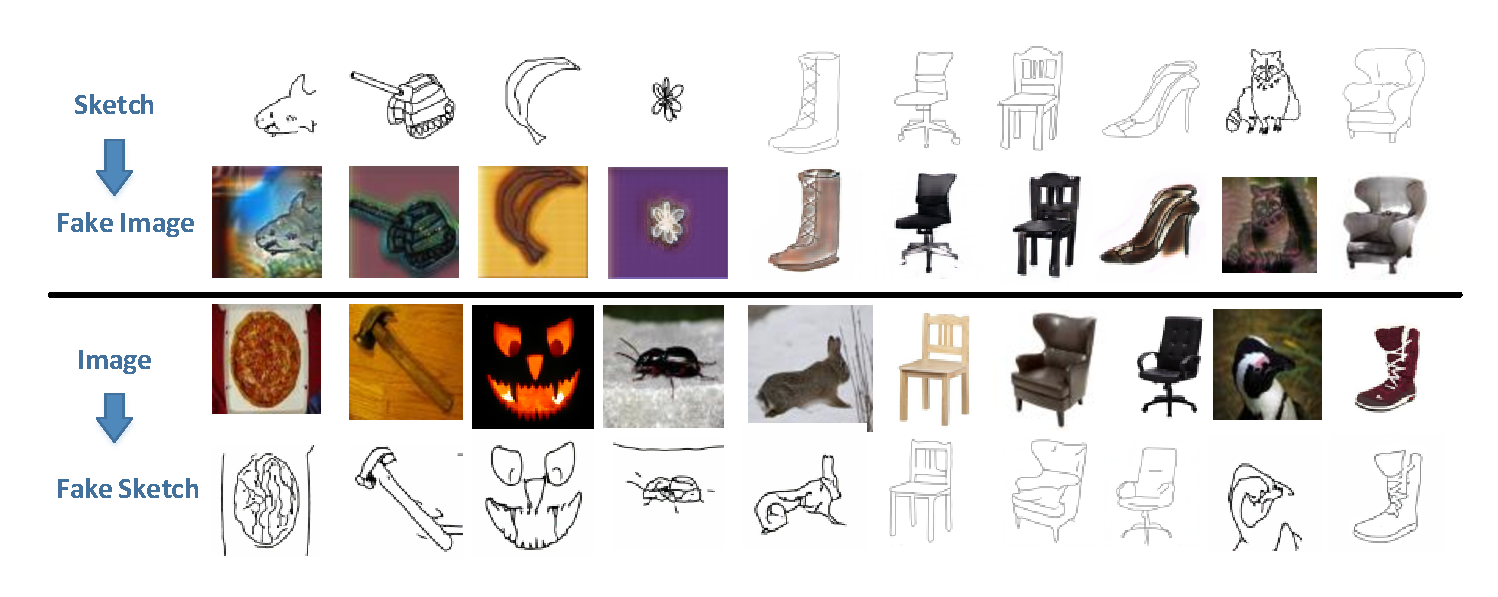
\includegraphics[width = 0.9\textwidth]{figures/gan_results.pdf}
    \vspace{-3ex}
    \caption{Visualization of our domain-migration networks. The first two rows are sketch-to-image results and the last two rows are image-to-sketch results, which indicates that our domain-migration networks are capable to transfer domains from both directions.}
    \label{fig:gan-figure}
\end{figure*}

\begin{table*}[t]
%\tiny
%\vspace{-1ex}
\begin{center}
%\footnotesize
\newcommand{\tabincell}[2]{\begin{tabular}{@{}#1@{}}#2\end{tabular}}
\caption{Effectiveness (MAP/accuracy with 128-bit) of different components (Sketchy for category-level SBIR and QMUL-Shoes for fine-grained SBIR).  }

\resizebox{0.9\textwidth}{!}{
\begin{tabular}{c|c|c|c}
  \hline
 \multirow{2}{*}{\textbf{Methods}} &\multirow{2}{*}{\tabincell{c}{\textbf{Category-level}\\ \textbf{MAP (Sketchy)}}} & \multicolumn{2}{c}{\textbf{Fine-grained acc. (QMUL-Shoes)}}\\
\cline{3-4}
 & &\qquad \quad \textbf{top-1} ~\qquad \qquad& \textbf{top-10} \\

  \hline
  \hline
  without $\mathcal{L}_{c}$  & 0.727 & - & - \\
  without $\mathcal{L}_{q}$ & 0.104 & - & -  \\
  without $\mathcal{L}_{gan}$ & 0.221 & 0.226 & 0.671\\
  \cline{1-4}
  without attention layer & 0.798 & 0.335 & 0.823\\
  \cline{1-4}
  Linear mix-up  &0.782 &0.282&0.744\\
  Concatenation mix-up &0.642 &0.182&0.654\\
  Kronecker product mix-up &0.735 &0.242&0.704\\
  \cline{1-4}
  Embed images into sketch domain  &0.310 & 0.263&0.791  \\
   \hline
   %the $\mathbf{H}\left ( G_I\left ( S_i \right );\bm{\theta}_H \right )$ and $\mathbf{H}\left ( I_i^+;\bm{\theta}_H \right )$
%Our model GDH 32bit &0.562 &0.948\\
%Our model GDH 64bit &0.748 &\textbf{1.00}\\
Our model GDH @ 128-bit (binary) &\textbf{0.811} & \textbf{0.357} & \textbf{0.843}\\

  \hline
  \end{tabular}
  }
\label{table:t4}
\end{center}
\vspace{-4ex}
\end{table*}

\section{Conclusion}
In this paper, we proposed a Generative Domain-migration Hashing method for both category-level and fine-grained SBIR tasks. Instead of mapping sketches and natural images into a common space, GDH for the first time employs a generative model that migrates sketches to their indistinguishable counterparts in the natural image domain. Guided by the adversarial loss and the cycle consistency loss, robust hashing codes for both real and synthetic images (\emph{i.e., migrated from sketches}) can be obtained with an end-to-end multi-task learning framework that does not rely on the pixel-level alignment between cross-domain pairs. We additionally integrated an attention layer to effectively suppress the background information and guide the learning process of GDH to concentrate on the most critical regions. Extensive experiments  on large-scale datasets demonstrated the consistently balanced superiority of GDH in terms of efficiency, memory costs and performance on both category-level and fine-grained SBIR tasks. GDH also outperformed the best-performing hashing-based SBIR method DSH \cite{LiuSSLS17} by up to $20.5\%$ on the TU-Berlin Extension dataset, and up to $26.4\%$ on the Sketchy dataset respectively. 



\bibliographystyle{splncs}
\bibliography{Ref}
\end{document}




